\documentclass[conference]{IEEEtran}
\IEEEoverridecommandlockouts
% The preceding line is only needed to identify funding in the first footnote. If that is unneeded, please comment it out.

\usepackage{cite}
\usepackage{amsmath,amssymb,amsfonts}
\usepackage{algorithmic}
\usepackage{graphicx}
\usepackage{textcomp}
\usepackage{xcolor}
\usepackage{needspace}

\def\BibTeX{{\rm B\kern-.05em{\sc i\kern-.025em b}\kern-.08em
    T\kern-.1667em\lower.7ex\hbox{E}\kern-.125emX}}

\usepackage{url}




% Reduce space around figures and tables
\setlength{\textfloatsep}{4pt}
\setlength{\floatsep}{5pt}
\setlength{\intextsep}{5pt}

% Reduce caption spacing
\setlength{\abovecaptionskip}{3pt}
\setlength{\belowcaptionskip}{0pt}

% Reduce spacing around equations
\setlength{\abovedisplayskip}{4pt}
\setlength{\belowdisplayskip}{4pt}

\bstctlcite{IEEEexample:BSTcontrol}

\begin{document}
\bstctlcite{IEEEexample:BSTcontrol}

\title{A Machine-Learning Analysis of the Higgs Boson in the $H \rightarrow ZZ^{*} \rightarrow 4\ell$ Channel\\}

\author{\IEEEauthorblockN{Student: Mane Papoyan}
\IEEEauthorblockA{\textit{Akian College of Science and Engineering} \\
\textit{American University of Armenia}\\
Yerevan, Armenia \\
papoyanmane2@gmail.com}
\and
\IEEEauthorblockN{Supervisor: Houry Keoshkerian}
\IEEEauthorblockA{\textit{Akian College of Science and Engineering} \\
\textit{American University of Armenia}\\
Yerevan, Armenia \\
hkeoshkerian@aua.am}
}
\maketitle

\begin{abstract}
We present a machine-learning analysis of the Higgs boson in the $H \rightarrow ZZ^{*} \rightarrow 4\ell$ channel using the ATLAS Open Data 2025 release at $\sqrt{s} = 13~\mathrm{TeV}$ $(36.6~\mathrm{fb}^{-1})$. The aim is to investigate whether the Higgs boson can be identified using machine learning. Seven classification algorithms are trained on simulated Monte Carlo data and then applied to the real ATLAS data to extract the signal. The two most consistent models, XGBoost and LightGBM, reach evidence-level significance under two independent background-estimation methods, yielding $Z = 4.70 \pm 1.35$ for XGBoost, and $Z = 5.08 \pm 1.50$ for LightGBM. Evidence for the Higgs boson is observed in two independent classifiers with consistent results across both methods.
\end{abstract}

\begin{IEEEkeywords}
ATLAS Open Data, Higgs boson, machine learning, particle physics
\end{IEEEkeywords}

\section*{Introduction}

The Standard Model of particle physics is the theoretical framework that describes the fundamental particles of nature and the forces governing their interactions. It classifies elementary particles into fermions, which make up the physical matter of the universe, and bosons (e.g., photons, W and Z bosons, and gluons), which mediate how those matter particles interact with each other. While the Standard Model successfully explains many behaviors and properties of particles, scientists have long wondered how particles acquire their mass. The answer to this question lies in the Higgs boson, an elementary particle in physics, the quantum excitation of the Higgs field, which gives other elementary particles their mass through their interactions with it. It was discovered in 2012 as a result of the ATLAS experiments at CERN's LHC (Large Hadron Collider), having been predicted decades earlier. This discovery completed the Standard Model of particle physics and confirmed how elementary particles acquire their mass. Since then, the Higgs boson has been studied in much greater detail, measuring its mass to be approximately $125~\mathrm{GeV}$ and its properties to be consistent with the predictions of the Standard Model.

Once produced in high-energy collisions, the Higgs boson is highly unstable and immediately decays into lighter particles. There are several possible decay paths, known as decay channels, each of which produces a distinct combination of final-state particles such as two photons, two W bosons, a pair of b-quarks, or two Z bosons. The likelihood of each channel is well predicted theoretically. In this work, we focus on the $H \rightarrow ZZ^{*} \rightarrow 4\ell$ channel of Higgs physics: the Higgs boson decays into a pair of Z bosons, and each Z then decays into two leptons (either electrons or muons), giving four leptons in the final state as shown in Fig.~1. This channel is rare, accounting for only about $2.6\%$ of all Higgs decays, but its final state is fully reconstructable, its detector signature is very clean, and its background, dominated by the non-resonant $ZZ^{*}$ continuum, with smaller contributions from $Z+$jets and $t\bar{t}$ processes, is well understood; hence the nickname ``golden channel''~\cite{ATLAS2012discovery,{ATLAS_Run2_2019}.

 \begin{figure}[htbp]
    \centering
    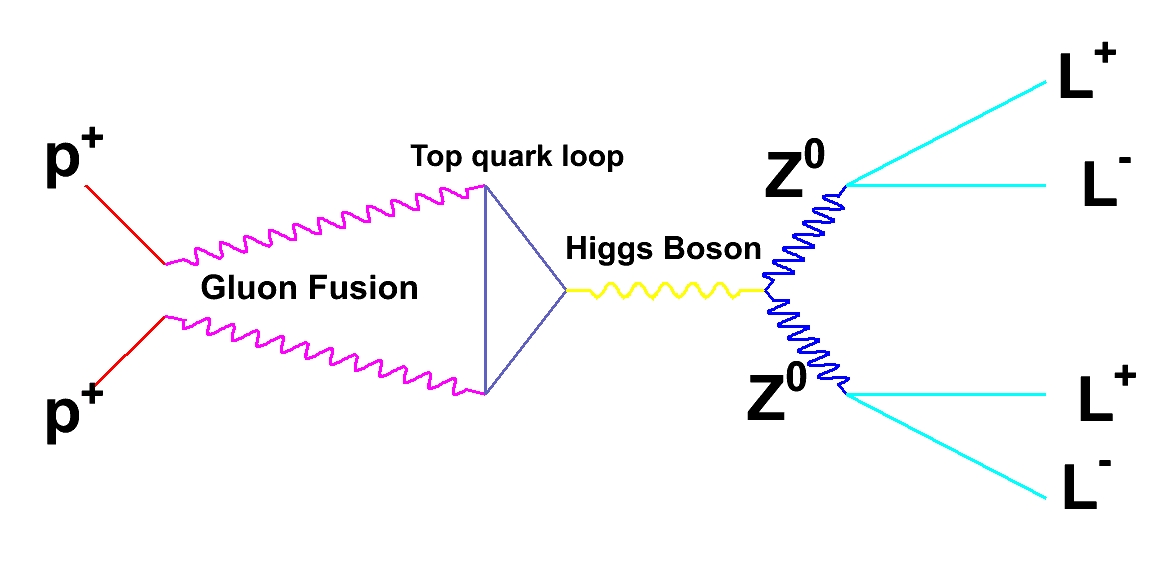
\includegraphics[width=0.3\textwidth]{Figures/feynman_diagram.png}
    \caption{ Four-lepton ”Golden” channel}
    \label{fig:Four_lepton channel}
\end{figure}

Despite the rapid growth of machine learning across the sciences, its use in particle physics, and in Higgs physics in particular, remains underdeveloped relative to what is possible. Within the large ATLAS and CMS collaborations, machine learning is typically embedded as one component of a much larger statistical framework rather than asked to identify a signal on its own. Outside of these collaborations, the standalone machine-learning literature on Higgs classification has concentrated almost exclusively on the $H \rightarrow \tau\tau$ channel, and the great majority of these studies evaluate their classifiers only on simulated Monte Carlo events, never carrying them through to a real-data test. The 2025 ATLAS Open Data release , which contains both real ATLAS collision data and the corresponding Monte Carlo samples, provides the dataset needed to test whether a classifier trained only on simulation can identify the Higgs boson when applied directly to real collision data \cite{ATLASOpenData2020}.

\section{Problem Statement and Research Question}
The problem addressed in this work is the absence of a standalone machine-learning benchmark for the $H \rightarrow ZZ^{*} \rightarrow 4\ell$ Higgs decay channel and the lack of real-data testing in the broader standalone Higgs-classification literature. The $H \rightarrow ZZ^{*} \rightarrow 4\ell$ channel, despite being the cleanest of all Higgs decay channels and the subject of decades of experimental work, has not been the subject of a standalone machine-learning benchmark comparable to what exists for $H \rightarrow \tau\tau$, and the broader question of whether a classifier trained only on Monte Carlo can identify the Higgs boson when applied directly to real ATLAS collision data is largely untested in the open literature. The specific research question is therefore:

\begin{quote}
Can a machine-learning classifier, trained only on simulated $H \rightarrow ZZ^{*} \rightarrow 4\ell$ events and applied directly to real ATLAS data, identify the Higgs boson on its own?
\end{quote}

To answer this question, two objectives are set. The first is to construct a controlled benchmark for the $H \rightarrow ZZ^{*} \rightarrow 4\ell$ channel by training seven classifiers, which are XGBoost, LightGBM, Random Forest, a multilayer perceptron, Logistic Regression, Quadratic Discriminant Analysis, and Gaussian Naive Bayes, under an identical 5-fold cross-validated protocol on 31 physics-motivated features. The second is to test whether the trained models generalize to real ATLAS data by applying each classifier to the 1,279 real ATLAS events in the 2025 Open Data release and computing the signal significance under two independent background-estimation methods.

\section*{Literature Study}
 
This section reviews the prior work that frames the present analysis. We organize the discussion into four threads: (a) the experimental discovery and measurement of the Higgs boson in the $H \rightarrow ZZ^{*} \rightarrow 4\ell$ channel, (b) the role of multivariate methods within official ATLAS and CMS analyses of this channel, (c) the broader landscape of standalone machine-learning studies of the Higgs boson, which is heavily concentrated on the $H \rightarrow \tau\tau$ channel and rarely touches the $4\ell$ final state, and (d) the ATLAS Open Data initiative as the vehicle that makes the present analysis possible.
 
\subsection{The {$H \rightarrow ZZ^{*} \rightarrow 4\ell$} Channel: From Discovery to Precision Physics}
 
The four-lepton final state has been central to Higgs physics since the 2012 discovery papers by the ATLAS and CMS collaborations~\cite{atlas2012observation,cms2012observation}. Early ATLAS searches at $\sqrt{s}=7~\mathrm{TeV}$ with $2.1~\mathrm{fb}^{-1}$ and later $4.8~\mathrm{fb}^{-1}$ of $pp$ collision data already exploited the four-lepton invariant mass $m_{4\ell}$ as the primary discriminant and established the methodological template, same-flavour opposite-sign lepton pairing, transverse-momentum staircase cuts, and on-shell/off-shell Z assignment, that subsequent analyses, including ours, continue to follow~\cite{atlas2012zz48fb,atlas2011zz21fb}.
 
After discovery, the field shifted to precision physics: the ATLAS measurement of the Higgs boson mass in $H \rightarrow ZZ^{*} \rightarrow 4\ell$ and $H \rightarrow \gamma\gamma$ with $36.1~\mathrm{fb}^{-1}$ at $13~\mathrm{TeV}$~\cite{atlas2018higgsmass}, and the more recent full Run-2 measurement using $139~\mathrm{fb}^{-1}$, which reports $m_H = 124.99 \pm 0.18~(\mathrm{stat.}) \pm 0.04~(\mathrm{syst.})~\mathrm{GeV}$~\cite{atlas2023run2mass}. These analyses are the methodological state of the art for the channel and are built around a maximum-likelihood fit of the $m_{4\ell}$ spectrum, augmented by physics-motivated multivariate discriminants used for event categorization rather than for primary signal extraction. The Higgs boson, in these analyses, is identified by the combination of cut-based selection, kinematic-likelihood discriminants, and a statistical fit of the mass spectrum, not by the machine-learning model alone.
 
\subsection{Multivariate Methods Inside the Official ATLAS/CMS Analyses}
 
The $4\ell$ channel has long benefitted from physics-motivated multivariate discriminants. Avery et al.~\cite{avery2013mekd} introduced the MEKD code, which computes kinematic discriminants from full leading-order matrix elements (the matrix-element method, or MEM), and demonstrated its discrimination power against the irreducible $ZZ^{*}$ background as well as its sensitivity to spin and CP hypotheses. Their work also emphasises the importance of correctly treating identical-lepton permutations and interference effects when constructing angular observables, a subtlety that directly informs how we compute the five helicity-frame angles in our feature set. CMS analyses have since adopted MEM-based likelihood discriminants in measurements of Higgs boson properties and the off-shell width~\cite{cms2021higgs4l}.
 
On the machine-learning side, the official ATLAS $36.1~\mathrm{fb}^{-1}$ and $139~\mathrm{fb}^{-1}$ mass measurements~\cite{atlas2018higgsmass,atlas2023run2mass} use BDTs trained on kinematic inputs to bin events into BDT-response categories, which sharpens the per-category $m_{4\ell}$ resolution within the likelihood fit. In all of these cases, however, the multivariate model operates inside a larger analysis framework: it categorizes, refines, or extracts couplings from a signal that the analysis as a whole identifies through the $m_{4\ell}$ fit. None of these published works ask whether the classifier by itself would be sufficient to identify the Higgs.

\subsection{Standalone Machine-Learning Studies Are Concentrated on $H \to \tau\tau$, Not on $H \to 4\ell$}

 
The broader machine-learning-in-HEP literature has produced many standalone Higgs-classification studies, but they are overwhelmingly concentrated on the $H \rightarrow \tau\tau$ channel. The 2014 ATLAS Higgs Machine Learning Challenge~\cite{adambourdarios2015higgsml}, hosted on Kaggle, released a 30-feature simulated dataset for $H \rightarrow \tau\tau$ classification, and this dataset has since become the de facto benchmark for machine-learning Higgs studies. The two top-ranked solutions, Chen and He's XGBoost-based entry~\cite{chen2015higgsxgb} and Melis's deep-learning entry, are still the most widely cited demonstrations of gradient-boosted trees and DNNs in Higgs physics.
 
Subsequent works built on this benchmark include Lalchand's bagged-boosting variant~\cite{lalchand2020bdt}, Sadowski et al.'s deep-learning study of multiple $H \rightarrow \tau\tau$ decay modes, and Lasocha et al.'s comparison of DNNs, boosted trees, random forests, and SVMs for $H \rightarrow \tau\tau$ CP-state classification~\cite{lasocha2018cp}. The Fair Universe HiggsML Uncertainty Challenge~\cite{bhimji2024fairuniverse}, launched in 2024, again uses an $H \rightarrow \tau\tau$ dataset. The same pattern holds for the foundational deep-learning paper of Baldi, Sadowski, and Whiteson~\cite{baldi2014deeplearning}: although it is often described as a ``Higgs benchmark,'' the dataset is in fact a simulated $H \rightarrow WW$-like process with two leptons and missing transverse energy, not a four-lepton final state.
 
To our knowledge, the $H \rightarrow ZZ^{*} \rightarrow 4\ell$ channel has not been the subject of a comparable standalone machine-learning benchmark. The few works that do involve machine learning in the $4\ell$ final state either sit inside official ATLAS or CMS analyses~\cite{atlas2018higgsmass,atlas2023run2mass}, where the model is one component of a larger likelihood-fit framework, or explore non-standard computational approaches such as quantum-search algorithms for event selection rather than supervised classification~\cite{kim2021quantum}. Most existing educational analyses built on the ATLAS Open Data releases use simple rectangular cuts and visual inspection of the $m_{4\ell}$ spectrum as the analysis endpoint~\cite{evans2021atlasopendata}, and no published work has performed a systematic machine-learning rediscovery of the Higgs boson in the $H \rightarrow ZZ^{*} \rightarrow 4\ell$ channel using the educational release and a real-data test. A systematic comparison of multiple modern classifiers, XGBoost, LightGBM, Random Forest, neural networks, and classical methods, within a unified protocol on the $H \rightarrow ZZ^{*} \rightarrow 4\ell$ channel has not been published.
 
A second pattern across this literature, equally relevant to the present work, is that the great majority of standalone studies evaluate their classifiers only on simulated Monte Carlo events. The 2014 Higgs Machine Learning Challenge dataset is entirely simulated~\cite{adambourdarios2015higgsml}; the Baldi et al.\ benchmark is simulated~\cite{baldi2014deeplearning}; the Lalchand, Chen--He, and Sadowski et al.\ follow-ups all train and test on simulation~\cite{chen2015higgsxgb,lalchand2020bdt}. This is methodologically appropriate for benchmarking, simulation provides exact signal/background labels, but it leaves an important question unanswered: would a model trained on simulation actually identify the Higgs boson when applied to real collision data?
 
This question matters because the transition from simulation to data is non-trivial. Monte Carlo samples have known imperfections, mismodelled detector resolution, residual differences in pile-up profiles, approximate higher-order corrections, and a classifier that overfits to these artefacts can perform very differently on real events.
 
\subsection{Positioning of the Present Work}
 
Taken together, the literature reviewed above motivates the specific question this work addresses. The $4\ell$ channel is methodologically mature for cut-based and likelihood-fit analyses, but it has not been the subject of a standalone machine-learning benchmark comparable to the 2014 $H \rightarrow \tau\tau$ Challenge. Standalone machine-learning Higgs studies almost exclusively target $H \rightarrow \tau\tau$ and stop at Monte Carlo simulation, leaving open whether models actually generalize from simulation to real ATLAS data in a different channel.
 
The ATLAS Open Data 2025 release~\cite{atlas2025opendata} provides, for the first time, a packaged dataset suitable for a closed-loop machine-learning analysis in the $4\ell$ channel, training on simulation, testing on real data, at an integrated luminosity comparable to the original discovery. The present work is therefore not framed as a competition with the official ATLAS likelihood-fit measurement, which uses a much larger dataset and a more sophisticated statistical apparatus. Instead, it asks a complementary question: whether a machine-learning classifier, trained only on simulated $H \rightarrow ZZ^{*} \rightarrow 4\ell$ events and applied directly to real ATLAS data, can identify the Higgs boson on its own.

\section*{Methodology}

\section{The ATLAS Detector}
The ATLAS detector is one of the main experiments at the LHC. It is designed to record the products of the high-energy proton-proton collisions with nearly \(4\pi\) coverage in solid angle. It consists of several concentric layers, each specialized for a different type of measurement: an inner tracking system reconstructs the trajectories of charged particles inside a \(2 \, \mathrm{T}\) magnetic field, electromagnetic and hadronic calorimeters measure the energies of electrons, photons, and hadrons, and an outer muon spectrometer identifies muons and measures their momenta. A multi-level trigger system selects the most physically interesting events in real time from the much larger collision rate, reducing the data volume to a manageable level for analysis \cite{atlas2018higgsmass}.

\section{Data and Simulated Samples}
The data used in this work were released in 2025 by the ATLAS Collaboration as an updated and expanded proton-proton (\(pp\)) collision dataset to the public for educational use. They were recorded by the ATLAS detector at the LHC during 2015--2016 at a centre-of-mass energy of \(\sqrt{s} = 13 \, \mathrm{TeV}\), corresponding to an integrated luminosity of approximately \(36.6 \, \mathrm{fb}^{-1}\). Alongside the real data, the release provides a set of Monte Carlo simulated samples for the relevant processes, used to model the expected distributions of both the \(H \rightarrow ZZ^{*} \rightarrow 4\ell\) signal and the main background contributions, which include the irreducible \(ZZ^{*} \rightarrow 4\ell\) continuum and the reducible \(Z+\mathrm{jets}\), \(t\bar{t}\), \(t\bar{t}+V\), and triboson (\(VVV\)) processes. The samples are distributed as ROOT files, which are a columnar data format widely used in high-energy physics, in a simplified version of the corresponding research-grade release of 2024. They are accessed through the \texttt{atlasopenmagic} Python package, which provides the data and simulation samples as awkward arrays for direct use in a Python analysis \cite{ATLASOpenData2020}.

\section{Preselection cuts}
The data and Monte Carlo samples are loaded through the \texttt{exactly4lep} skim of the Open Data release, which pre-selects events containing exactly four reconstructed leptons. Additionally, the four leptons must form a same-flavor, opposite-sign pairing (4e, 4$\mu$, or 2e2$\mu$), and the sum of their charges must be zero, therefore in principle resulting in two Z boson candidates.

After the skim and the flavour pairing, we impose constraints on the lepton transverse momenta $p_T$, defined as the projection of the momentum vector onto the plane transverse to the beam direction. Ordering the four leptons in descending $p_T$, the selection criteria are summarized in Table~\ref{tab:pt_cuts}. This ``staircase'' requirement suppresses backgrounds in which one or more leptons are soft, as is typical for $Z+$jets and $t\bar{t}$ events.

After the full preselection, the unweighted Monte Carlo sample contains 226{,}168 signal events and 12{,}436 background events, with 1{,}279 events observed in the real data. \cite{atlas2018higgsmass}

\begin{table}[htbp]
\centering
\caption{Transverse momentum selection requirements for leptons.}
\label{tab:pt_cuts}
\begin{tabular}{c c}
\hline
Lepton & Requirement \\
\hline
$l_1$ & $p_T > 20~\mathrm{GeV}$ \\
$l_2$ & $p_T > 15~\mathrm{GeV}$ \\
$l_3$ & $p_T > 10~\mathrm{GeV}$ \\
$l_4$ & $p_T > 7~\mathrm{GeV}$ \\
\hline
\end{tabular}
\end{table}


\section{$Z_1$ and $Z_2$ Reconstruction}
\label{sec:Z1Z2_reco}
Given four leptons in an event, there are up to three distinct ways to combine them into two pairs: $(\ell_1\ell_2)(\ell_3\ell_4)$, $(\ell_1\ell_3)(\ell_2\ell_4)$, and $(\ell_1\ell_4)(\ell_2\ell_3)$. Of these, only the pairings that produce two same-flavour, opposite-sign dilepton pairs are valid as Z-boson candidates. Among the valid pairings, the one whose dilepton invariant mass comes closest to the nominal Z mass, $M_Z = 91.2~\mathrm{GeV}$, is chosen as the on-shell Z candidate, labelled $Z_1$, while the remaining pair is taken as the off-shell candidate, $Z_2$. This pairing prescription matches the standard ATLAS convention for this channel, stating that in a real $H \rightarrow ZZ^{*} \rightarrow 4\ell$ event with $m_H = 125~\mathrm{GeV}$, only one Z can be on-shell, because there is not enough mass available to produce two real Z bosons simultaneously.

The four-lepton system formed by combining $Z_1$ and $Z_2$ is the Higgs boson candidate, and its invariant mass $m_{4\ell}$ is the most important kinematic variable in the analysis: a true Higgs decay produces a sharp peak at $m_{4\ell} \approx 125~\mathrm{GeV}$, while background processes produce a smoothly varying distribution with no such peak as shown in Fig.~\ref{fig:four_lepton_mass}. The dilepton invariant masses $m(Z_1)$ and $m(Z_2)$, together with the kinematic and angular quantities that can be derived from the Z-system rest frames, are passed to the classifiers as input features.

\begin{figure}[htbp]
    \centering
    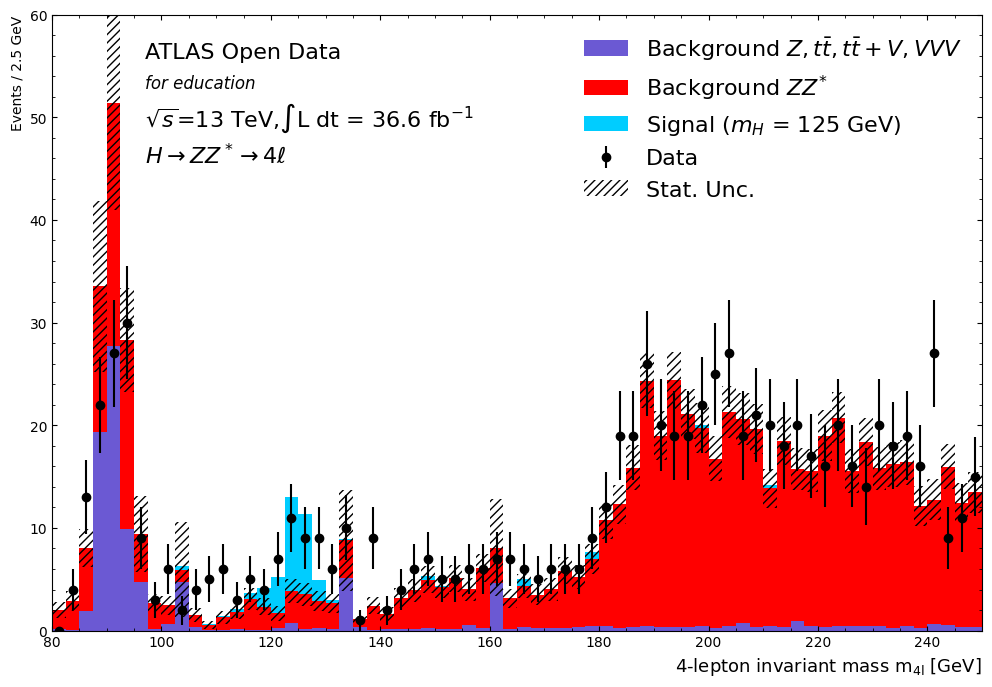
\includegraphics[width=0.4\textwidth]{Figures/m4l.png}
    \caption{Invariant mass distribution of the four-lepton system $m_{4\ell}$. A Higgs boson signal as a peak around 125 GeV.}
    \label{fig:four_lepton_mass}
\end{figure}


\section{Event weighting}
Next, we apply per-event Monte Carlo weights to scale the simulated samples to the dataset’s integrated luminosity of $36.6~\mathrm{fb}^{-1}$, in order for them to be directly comparable. The cross-section weight is given by

\begin{equation}
w_{\sigma} =
\frac{
\mathcal{L} \cdot \sigma \cdot \eta \cdot k \cdot w_{\mathrm{MC}}
}{
\sum_i w_i
}
\label{eq:xsec_weight}
\end{equation}

where $\mathcal{L}$ is the integrated luminosity of the dataset ($36.6~\mathrm{fb}^{-1}$), $\sigma$ is the process cross-section, $\eta$ is the filter efficiency at generator level, $k$ is the higher-order correction factor (k-factor), $w_{\mathrm{MC}}$ is the generator-level event weight, and the denominator $\sum_i w_i$ is the sum of generator weights across the full sample. The values of $\sigma$, $\eta$, $k$, and $w_{\mathrm{MC}}$ are stored as per-event variables in the Open Data ROOT files and are different for each Monte Carlo process.

Each event weight is additionally multiplied by the per-event scale factors provided with the Open Data release: pile-up, electron reconstruction and identification, muon reconstruction and identification, and lepton trigger corrections, according to
\begin{equation}
w_{\mathrm{total}} =
w_{\sigma} \cdot
SF_{\mathrm{pileup}} \cdot
SF_{\mathrm{electron}} \cdot
SF_{\mathrm{muon}} \cdot
SF_{\mathrm{trigger}}
\label{eq:total_weight}
\end{equation}

The final per-event weight $w_{\mathrm{total}}$ is the quantity used everywhere downstream for histograms, yields, and significance calculations.

After applying this weighting on top of the full preselection chain, the expected signal yield is $30.4 \pm 1.3$ events, the dominant $ZZ^{*}$ continuum yield is $1067.1 \pm 18.2$ events, and the reducible backgrounds ($Z+$jets, $t\bar{t}$, $t\bar{t}+V$, triboson) contribute $127.6 \pm 16.3$ events, giving a total expected background of $1194.7 \pm 24.4$ events. This shows a major difference compared to the unweighted Monte Carlo sample containing 226{,}168 signal events and 12{,}436 background events. The resulting signal-to-background ratio of approximately $1:40$ reflects the realistic regime in which the analysis must be carried out, and explains why even the four-lepton channel remains challenging in practice despite its clean detector signature.


\begin{table}[htbp]
\centering
\small
\caption{Signal and background yields}
\label{tab:yield_preselection}

\resizebox{0.48\textwidth}{!}{
\begin{tabular}{l c c}
\hline
Process & Raw Yield & Weighted Yield \\
\hline
$H \rightarrow ZZ^{*} \rightarrow 4\ell$ (Signal) & 226{,}168 & $30.43 \pm 1.33$ \\
$ZZ^{*} \rightarrow 4\ell$ (Irreducible Bkg) & 6{,}364 & $1067.08 \pm 18.15$ \\
Reducible Backgrounds & 6{,}033 & $127.61 \pm 16.32$ \\
\hline
Total Background & 12{,}436 & $1194.69 \pm 24.41$ \\
\hline
Data & & 1{,}279\pm 35.8 \\
\hline
\end{tabular}
}
\end{table}

\section{Feature Engineerin}
\subsection{The Kinematic Variables}

Each event is reconstructed from the four-momenta of the four leptons in the final state, as stored in the ROOT files (\texttt{lep\_pt}, \texttt{lep\_eta}, \texttt{lep\_phi}, \texttt{lep\_e}, together with \texttt{lep\_charge} and \texttt{lep\_type}) \cite{CMS2025Higgs4l}. From these inputs we construct 31 physics-motivated features capturing the kinematic and angular structure of the $H \rightarrow ZZ^{*} \rightarrow 4\ell$ topology, organized into seven groups:

\begin{enumerate}[(i)]
    \item the reconstructed Z-boson masses and transverse momenta,
    $m_{Z_1}, m_{Z_2}, p_{T}^{Z_1}, p_{T}^{Z_2}$;
    
    \item the transverse momentum of the four-lepton system,
    $p_{T}^{4\ell}$;
    
    \item per-lepton kinematic variables after Z-boson assignment ($p_T$ and $\eta$ for each lepton, eight features);
    
    \item five helicity-frame angles,
    $\theta_1, \theta_2, \Theta, \Phi, \Phi_1$,
    defined following the convention of Gao \textit{et al.}~\cite{Gao_2010};
    
    \item angular separation observables, two intra-Z $\Delta\phi$ values and four cross-pair $\Delta R$ values;
    
    \item scalar sums of the lepton transverse momenta within each Z; and
    
    \item event-level quantities
    $N_{\mathrm{jet}}$,
    $E_{T}^{\mathrm{miss}}$,
    and
    $\phi_{\mathrm{miss}}$.
\end{enumerate}


\textbf{1) Z-boson Pair Reconstruction:} The pairing prescription is described in Section~\ref{sec:Z1Z2_reco}. In practice, pair invariant masses are computed by summing four-momenta using the \texttt{vector} library; events with no SFOS pairing are dropped, and the transverse momenta $p_T^{Z_1}$ and $p_T^{Z_2}$ are obtained from each pair's summed four-momentum.

\textbf{2) Four-lepton Transverse Momentum:} $p_T^{4\ell}$ is the magnitude of the \textit{vector} sum of the four lepton transverse momenta, making it sensitive to angular correlations among the leptons (unlike a scalar sum).


\textbf{3) Per-lepton Kinematic Variables After Z Assignment:}Within each Z, the two leptons are ordered by transverse momentum into ``leading'' ($\ell_1$) and ``subleading'' ($\ell_2$) slots, giving four ordered positions:

\[
(Z_1,\ell_1),\;
(Z_1,\ell_2),\;
(Z_2,\ell_1),\;
(Z_2,\ell_2).
\]

For each we record $p_T$ and $\eta$ (eight features total). This ordering is preserved throughout the pipeline so the cross-pair angular variables (\S5) refer to well-defined slots.


\textbf{4) Helicity-frame Angles:}The five helicity angles characterize the angular distribution of the decay and are sensitive to the spin-parity quantum numbers of the parent resonance~\cite{Gao_2010}. They are computed by explicit Lorentz boosts of the lepton four-momenta into the relevant rest frames, with boost velocity

\[
\vec{\beta} = \frac{\vec{P}}{E}
\]

and Lorentz factor

\[
\gamma = \frac{1}{\sqrt{1-\beta^2}}
\]

for a target frame of four-momentum
$P = (E,\vec{P})$.

\paragraph{$\theta_1,\theta_2$:}

For each Z, the negative lepton and the four-lepton (Higgs) four-momentum are boosted into that Z's rest frame. $\theta_k$ is the angle between the boosted negative-lepton direction and the negative of the boosted Higgs direction:

\[
\cos\theta_k
=
\hat{p}_{\ell^-, Z_k\text{-RF}}
\cdot
\left(
-\hat{p}_{H, Z_k\text{-RF}}
\right).
\]

\paragraph{$\Theta$:}

The $Z_1$ four-momentum is boosted into the Higgs rest frame, and $\Theta$ is the angle between the boosted $Z_1$ direction and the beam axis $\hat{z}$ (taken as the laboratory beam axis).

\paragraph{$\Phi$:}

The signed angle between the two Z decay planes in the Higgs rest frame, with each decay plane defined by the cross product

\[
\vec{n}_k
=
\hat{p}_{\ell_k^-}
\times
\hat{p}_{\ell_k^+},
\]

is

\[
\Phi
=
\mathrm{sgn}
\left(
\vec{n}_1
\cdot
(\vec{n}_2 \times \hat{p}_{Z_1})
\right)
\,
\arccos
\left(
\hat{n}_1 \cdot \hat{n}_2
\right)
\in [-\pi,\pi].
\]

\paragraph{$\Phi_1$:}

The signed angle between the $Z_1$ decay plane and the plane spanned by $\vec{p}_{Z_1}$ and the beam axis, defined analogously to $\Phi$.

Dot products are clipped to $[-1,1]$ before $\arccos$ to guard against floating-point round-off.

\textbf{5) Angular Separation Observables:} In the laboratory frame, the opening azimuthal separation is wrapped to $[0,\pi]$, and

\[
\Delta R
=
\sqrt{
\Delta\eta^2 + \Delta\phi^2
}.
\]

We retain two intra-Z $\Delta\phi$ values,
$\Delta\phi_{Z_1}$ and $\Delta\phi_{Z_2}$,
and four cross-pair $\Delta R$ values between leptons of different Z candidates --- corresponding to the $(\mathrm{lead},\mathrm{sub}) \times (\mathrm{lead},\mathrm{sub})$ combinations of $Z_1$ and $Z_2$ leptons. These cross-pair $\Delta R$ values are constructed \textit{after} Z assignment so the four slots remain consistent across events.

\textbf{6) Scalar Transverse-momentum Sums:} For each Z we form the arithmetic sum

\[
\Sigma p_T^{Z_k}
=
p_T^{Z_k,\ell_1}
+
p_T^{Z_k,\ell_2}.
\]

Unlike $p_T^{Z_k}$ (the vector sum, sensitive to lepton opening angle), the scalar sum measures the overall hardness of each Z's decay independently of its decay-plane orientation.


\textbf{7) Event-level Observables} The jet multiplicity
$N_{\mathrm{jet}}$,
missing transverse energy
$E_T^{\mathrm{miss}}$,
and its azimuthal angle
$\phi_{\mathrm{miss}}$
are taken directly from the input ROOT files. These help separate the Higgs signal from reducible backgrounds with genuine neutrinos or extra hadronic activity (e.g.\ $t\bar{t}$ and $Z+$jets).

Histograms of all 31 features are then plotted to compare signal and background distributions; Fig.~3, for example, shows the transverse momentum distributions of the four leptons.

\begin{figure}[htbp]
    \centering
    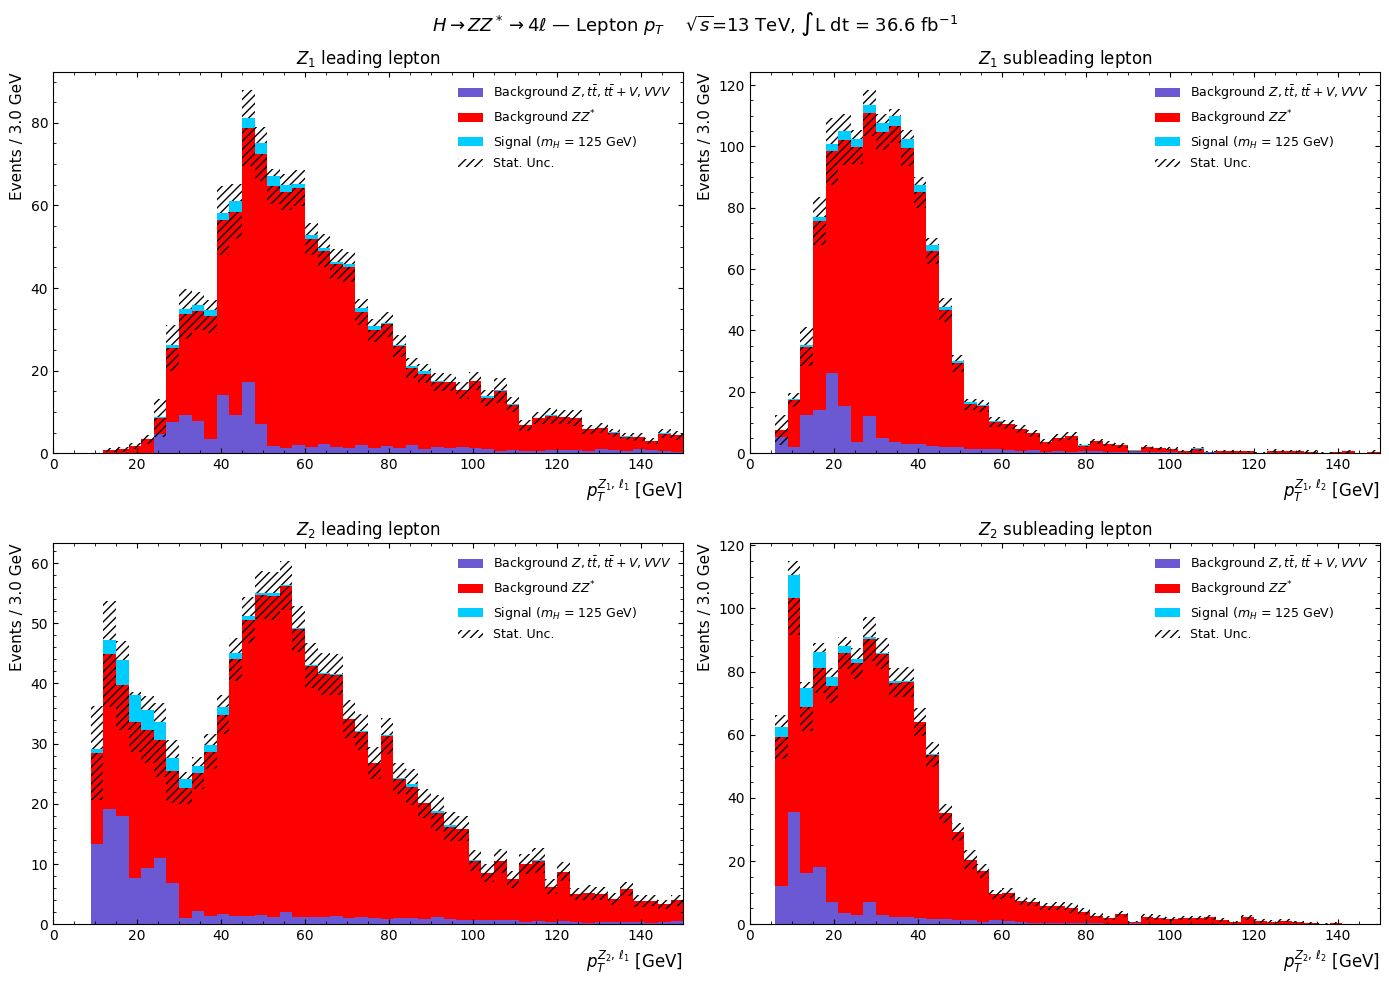
\includegraphics[width=0.4\textwidth]{Figures/pt_leptons.png}
    \caption{Transverse momentum distributions of the four leptons.}
    \label{fig:pt_leptons}
\end{figure}

By examining the shapes differences in these histograms for signal and background samples, we gain physical insight into how each feature can contribute to the overall classification task.


\subsection{Feature ranking and selection}
To select a robust input set without overfitting feature choice to any single criterion, the separation power ranking method has been applied to the training set only,

\begin{equation}
\delta^{2} = \frac{1}{2}\sum_{i}\frac{(s_{i}-b_{i})^{2}}{s_{i}+b_{i}},
\label{eq:separation_power}
\end{equation}
shown in Fig.~\ref{fig:separation_power}, computed over 50 bins per feature.

\begin{figure}[htbp]
    \centering
    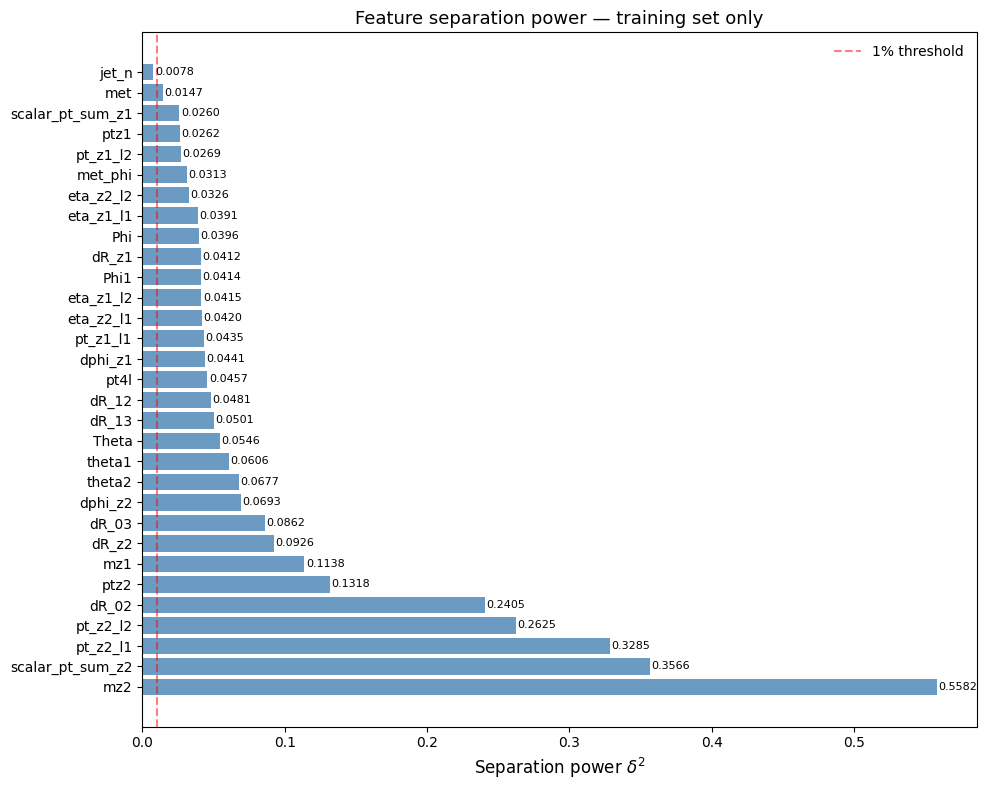
\includegraphics[width=0.85\columnwidth]{Figures/separation_power.png}
    \caption{Feature ranking based on separation power $\delta^2$. Higher values indicate stronger discrimination between signal and background.}
    \label{fig:separation_power}
\end{figure}

For each ranking, feature pairs with $|\rho| \geq 0.7$, as shown in the correlation matrix in Fig.~\ref{fig:corr_matrix} for the signal sample, are pruned by dropping the lower-ranked feature in each pair. The final feature set has 20 variables used for all downstream classifiers.
\begin{figure}[htbp]
    \centering
    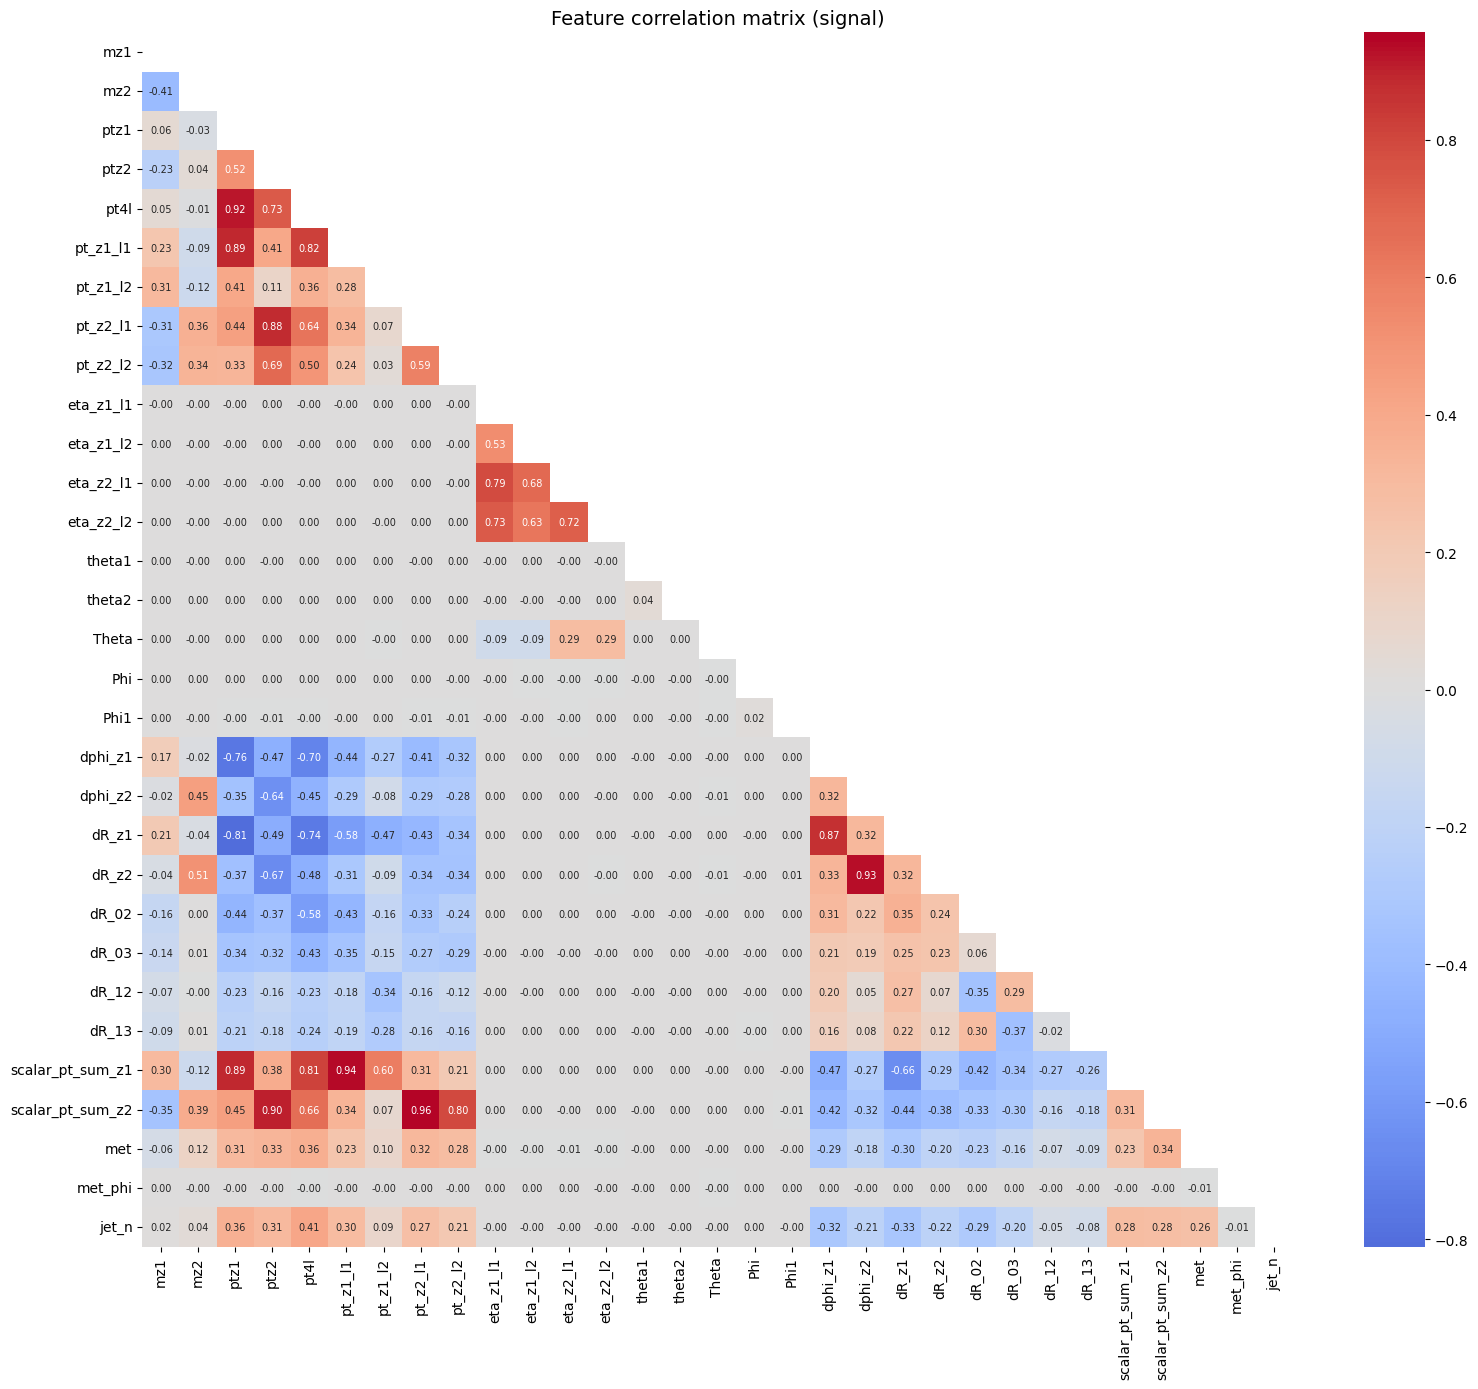
\includegraphics[width=0.85\columnwidth]{Figures/correlation_matrix.png}
    \caption{Pearson correlation matrix of the signal sample. Highly correlated feature pairs with $|\rho| \geq 0.7$ are used for feature pruning in the selection procedure.}
    \label{fig:corr_matrix}
\end{figure}

\section{ML Classifier Training}

The full analysis pipeline is organized as follows. Raw ROOT files are preselected, reweighted to the integrated luminosity of $36.6~\mathrm{fb}^{-1}$, and reduced to a 20-feature representation. The resulting Monte Carlo dataset is split into five stratified folds, on which seven classifiers are trained and scored out-of-fold under an identical protocol. The OOF scores fix a uniform working point at $0.65$, which is then applied both to the Monte Carlo sample and to the 1,279 real ATLAS events, where the signal significance is computed under two independent background-estimation methods.

The seven classifiers are XGBoost, LightGBM, Random Forest, a multilayer perceptron (MLP) implemented in Keras, Logistic Regression, Quadratic Discriminant Analysis (QDA), and Gaussian Naive Bayes (GaussianNB). They are chosen to span a deliberately broad methodological range, two gradient-boosted decision-tree implementations (XGBoost, LightGBM), a bagged-tree ensemble (Random Forest), a feed-forward neural network (MLP), a generalized linear model (Logistic Regression), and two generative classifiers based on Gaussian assumptions on the feature distributions (QDA, GaussianNB), so that the comparison isolates the contribution of the modeling assumption from differences in training data, feature set, or evaluation procedure. Five-fold cross-validation is used in place of a single train/validation/test split so that every Monte Carlo event is scored by a model that did not see it during training, recovering the full simulation statistics for both training and evaluation while eliminating optimistic bias from train/test contamination.

Software and compute environment\footnote{The full pipeline is implemented in Python~3.11 and executed on Google Colab with a single CPU runtime (no GPU is used; the MLP is small enough that CPU training is faster than the GPU initialization overhead). The main libraries are NumPy, \texttt{awkward-array}, and \texttt{uproot} for I/O and array manipulation; the \texttt{vector} library for four-momentum operations and Lorentz boosts; \texttt{atlasopenmagic} for access to the ATLAS Open Data samples; \texttt{scikit-learn} for Random Forest, Logistic Regression, QDA, GaussianNB, cross-validation utilities, and the standard scaler; \texttt{XGBoost} and \texttt{LightGBM} for boosted-tree models; \texttt{TensorFlow/Keras} for the MLP; and \texttt{matplotlib} for plotting. End-to-end training of all seven classifiers under the 5-fold protocol completes in approximately 127 minutes on a standard Colab CPU runtime.}

\subsection{Cross-Validation and Out-of-Fold Evaluation}
 
All seven models are trained on Monte Carlo simulation and
evaluated under $5$-fold stratified cross-validation to obtain
out-of-fold (OOF) predictions for every event. Stratification
preserves the signal-to-background proportion in each fold,
which is essential given the strong class imbalance in the
unweighted Monte Carlo sample ($226{,}168$ signal vs.\ $12{,}436$
background events). The fold structure ensures that every event
is scored by a model that did not see it during training,
eliminating optimistic bias from train/test contamination and
allowing the full Monte Carlo statistics to be used for both
training and evaluation.
 
Within each outer fold, an additional $20\%$ of the training
events is held out as an internal validation set for the
boosted-tree models and the MLP, used exclusively for early
stopping. Input features are standardized to zero mean and unit
variance using a \texttt{StandardScaler} fit on the training
fold only; the same transformation is then applied to the
validation and test folds. Random Forest is exempt from
scaling, as decision-tree splits are invariant under monotone
feature transformations.
 
\subsection{Class Imbalance Handling}
 
Class imbalance, meaning the signal weights are substantially
smaller than the background weights after luminosity scaling
(the weighted signal-to-background ratio is approximately
$1:40$), is addressed by passing
\[
\texttt{positive-class weight scaling} \;=\;
\frac{\sum w_{\mathrm{bkg}}}{\sum w_{\mathrm{sig}}}
\]
to the boosted trees through the \texttt{scale\_pos\_weight}
parameter, and by using class-balanced sample weights for the
Random Forest, MLP, and Logistic Regression: each signal weight
is scaled upward by the same ratio, so that the total weight
of the signal class equals the total weight of the background
class during training. For QDA, which in its \texttt{scikit-learn}
implementation does not natively support sample weights, the
class balance is instead introduced through a weighted-bootstrap
resampling of each fold's training set, with the resampling
probability proportional to the per-event Monte Carlo weight.
GaussianNB is trained directly with the raw luminosity weights
via the \texttt{sample\_weight} argument, since its closed-form
estimators for the per-class means and variances accept weights
natively.
 
In all cases, the original luminosity weights, not the balanced
versions, are preserved for the evaluation metrics, so that all
reported AUCs, yields, and significances correspond to physically
meaningful event counts.
 
\subsection{Model Architectures and Hyperparameters}
 
The architectural and hyperparameter choices for the seven
classifiers are summarized in Table~\ref{tab:hyperparameters}.
The two boosted-tree models share the same base configuration,
$500$ estimators with a learning rate of $0.05$, row and column
subsampling rates of $0.8$, and early stopping with a patience
of $20$ iterations on the internal validation AUC, so that the
difference between them reflects the implementation rather than
the training budget.
 
\begin{table*}[t]
\centering
\caption{Hyperparameter settings for all seven classifiers.
All models are trained under a common $5$-fold stratified
cross-validation protocol on the same $20$ features.}
\label{tab:hyperparameters}
\small
\begin{tabular}{l l}
\hline
\textbf{Classifier} & \textbf{Settings} \\
\hline
XGBoost      & $n_{\mathrm{est}}=500$, max\_depth and min\_child\_weight tuned (see Table~\ref{tab:xgb_grid}), \\
             & learning\_rate $=0.05$, subsample $=0.8$, colsample\_bytree $=0.8$, $\gamma=0$, \\
             & $\lambda=1$, $\alpha=0$, \texttt{tree\_method}=hist, early\_stopping\_rounds $=20$ \\
\hline
LightGBM     & $n_{\mathrm{est}}=500$, max\_depth $=4$, num\_leaves $=15$, \\
             & learning\_rate $=0.05$, subsample $=0.8$, subsample\_freq $=1$, colsample\_bytree $=0.8$, \\
             & min\_child\_samples $=20$, $\lambda=1$, $\alpha=0$, early\_stopping\_rounds $=20$ \\
\hline
Random Forest & $n_{\mathrm{est}}=300$, max\_depth $=5$, min\_samples\_leaf $=5$, bootstrap $=$ True \\
\hline
MLP (Keras)  & layers $=[128,64,32]$ + $1$, activations: ReLU/ReLU/ReLU/sigmoid, \\
             & optimizer = Adam, learning\_rate $=10^{-3}$, loss = binary cross-entropy, \\
             & epochs (max) $=100$, batch\_size $=256$, early\_stopping patience $=10$ on val\_loss \\
\hline
Logistic Reg.& solver = lbfgs, max\_iter $=2000$, $C$ tuned over $\{10^{-3},10^{-2},10^{-1},1,10,10^{2}\}$, \\
             & inner $3$-fold CV used to select $C$, best $C=100$ \\
\hline
QDA          & reg\_param $=0.1$, weighted bootstrap resampling per fold \\
\hline
GaussianNB   & \texttt{scikit-learn} defaults; native \texttt{sample\_weight} used \\
\hline
\end{tabular}
\end{table*}
 
\subsubsection{Boosted Trees: XGBoost and LightGBM}
 
For XGBoost, the two hyperparameters with the largest impact on
generalization in this dataset, the maximum tree depth and the
minimum child weight, are tuned by a $5$-fold inner
cross-validated grid search over
\[
\begin{aligned}
\text{maximum tree depth} &\in \{3,4,5\}, \\
\text{minimum child weight} &\in \{1,5,10\}.
\end{aligned}
\]
Within each inner fold, the same internal validation split
(20\%, stratified) and early-stopping criterion are used as in
the outer loop, so that the number of trees is selected
adaptively for each hyperparameter combination rather than fixed
in advance. The remaining hyperparameters are held at the values
listed in Table~\ref{tab:hyperparameters}, since the learning
rate, subsampling rates, and regularization terms are already
in a well-behaved regime for this problem size and further
tuning produces no measurable improvement. The full grid-search
results, including the per-combination mean OOF AUC and its
fold-to-fold standard deviation, are reported in
Table~\ref{tab:xgb_grid}. The chosen combination is the one
with the highest mean inner AUC.
 
 
LightGBM is trained at a fixed configuration motivated by the
optimal XGBoost depth: \texttt{maximum depth}~$=4$ and
\texttt{maximum number of leaves}~$=15\approx 2^{\texttt{maximum depth}}-1$, with
\texttt{minimum samples per leaf}~$=20$ to suppress overfitting on
the small signal population. The early-stopping criterion is
identical to that of XGBoost. A separate LightGBM grid search
was not performed, since the two implementations differ
primarily in their tree-growth strategy (depth-wise vs.\
leaf-wise) and not in the meaning of the depth parameter, and
the LightGBM AUC at the matched configuration is already
within the bootstrap uncertainty of the tuned XGBoost result. You can see the further details and the results of the hyperparameter tuning in the appendices (Table~\ref{tab:auc_results}).
 
\subsubsection{Random Forest}
 
Random Forest is used with $300$ trees, a maximum depth of $5$,
and a minimum of $5$ samples per leaf. The shallow depth and
the per-leaf minimum are deliberately conservative: with the
luminosity-scaled signal yield of only $\sim 30$ events, deeper
trees rapidly memorize individual high-weight signal events and
inflate the in-sample AUC without improving the OOF score. The
number of trees is set well above the point of saturation;
beyond $\sim 200$ trees the OOF AUC changes by less than the
seed-to-seed variation.
 
\subsubsection{Multilayer Perceptron}
 
The MLP uses three hidden layers ($128$, $64$, and $32$ units)
with ReLU activations, a sigmoid output, and the Adam optimizer
with a learning rate of $10^{-3}$ and a binary cross-entropy
loss. Training runs for up to $100$ epochs in batches of
$256$ events and is stopped early on a validation-loss plateau
with a patience of $10$ epochs and best-weight restoration.
This architecture, of order $30{,}000$ trainable parameters,
is intentionally small relative to the size of the training
fold (more than $10^5$ events): a larger network does not
improve the OOF AUC and develops a visible train-validation
loss gap. The same architecture is rebuilt independently for
each of the five outer folds, with the fold-dependent random
seed $42+\text{fold\_idx}$ used to initialize the weights, so
that each fold's MLP is statistically independent of the others.
 
\subsubsection{Logistic Regression}
 
For Logistic Regression, the inverse regularization strength
is selected by a $6$-point inner cross-validated scan over
\[
C\in\{0.001,0.01,0.1,1.0,10.0,100.0\},
\]
using a $3$-fold inner stratified split on the training data
of each outer fold, evaluated with the raw luminosity weights
to obtain physics-correct AUCs. The optimal value is found to
be $C=100$, indicating that the data prefer a weak regularization
once the inputs are standardized and the class weights balanced.
The solver is \texttt{lbfgs} with a maximum of $2000$ iterations
to ensure convergence at the largest tested $C$.
 
\subsubsection{Quadratic Discriminant Analysis and GaussianNB}
 
QDA is used with a small covariance regularization of
$\texttt{reg\_param}=0.1$ to stabilize the inversion of the
per-class covariance matrices in feature directions of low
variance, and receives its sample weights through a
weighted-bootstrap resampling of each fold's training set, as
described above. GaussianNB is used with its \texttt{scikit-learn}
defaults after standard scaling of the input features, and uses
the per-event Monte Carlo weights directly through its native
\texttt{sample\_weight} argument. Both models retain their
generative form, $p(\mathbf{x}\mid y)$, and convert it into a
posterior $p(y\mid \mathbf{x})$ via Bayes' rule. Their
performance on this problem is therefore a direct test of
whether the joint distribution of the 20 input features can
plausibly be approximated as a (per-class) Gaussian, full
covariance for QDA and diagonal for GaussianNB.
 
\subsection{Number of Folds: Stability Study}
 
The choice of $k=5$ folds is motivated by a stability study in
which the analysis is repeated for
\[
k\in\{3,5,7,10\},
\]
holding all other hyperparameters and seeds fixed. For $k>5$,
the fold-to-fold standard deviation in AUC increases without a
corresponding improvement in either the mean AUC or the
downstream signal significance, indicating that beyond five
folds the additional partitioning produces noisier per-fold
estimates without recovering more usable training data. For
$k=3$, the per-fold training set is large enough to converge
the boosted-tree models, but the per-fold test set is too
small to give a stable significance, and the OOF estimate shows
visible drift from one repetition to the next. The value
$k=5$ is therefore retained as the working point for all seven
classifiers.
 
\subsection{Seed Stability}
 
A complementary seed-stability check repeats the $5$-fold
training with fifteen different random seeds for both the fold
partitioning and the model initialization, with the same seed
used for both within a given replicate. The resulting AUC
variation across seeds is below $0.005$ and the variation in
the downstream significance below approximately $3\%$,
confirming that the reported metrics are not artefacts of a
particular train/test partition. The seed scan is performed
on XGBoost, the model whose downstream significance is most
sensitive to the choice of partition; the spread is taken as
representative of the other classifiers, which use the same
fold structure.
 
\subsection{Per-Model AUC and Uncertainties}
 
Uncertainties on the per-model AUC are estimated using a
stratified bootstrap procedure with $1000$ resamples of the
OOF scores, drawn with replacement while preserving the
class-balance proportions and using the per-event luminosity
weights in both the resampling and the AUC computation. The
$95\%$ confidence interval is taken as the $2.5$th and
$97.5$th percentiles of the bootstrap AUC distribution. The
resulting OOF AUC values for the seven models are summarized
in the ROC-curve comparison shown in Fig.~6 and in
Table~\ref{tab:auc_results}.

\begin{figure}[htbp]
    \centering
    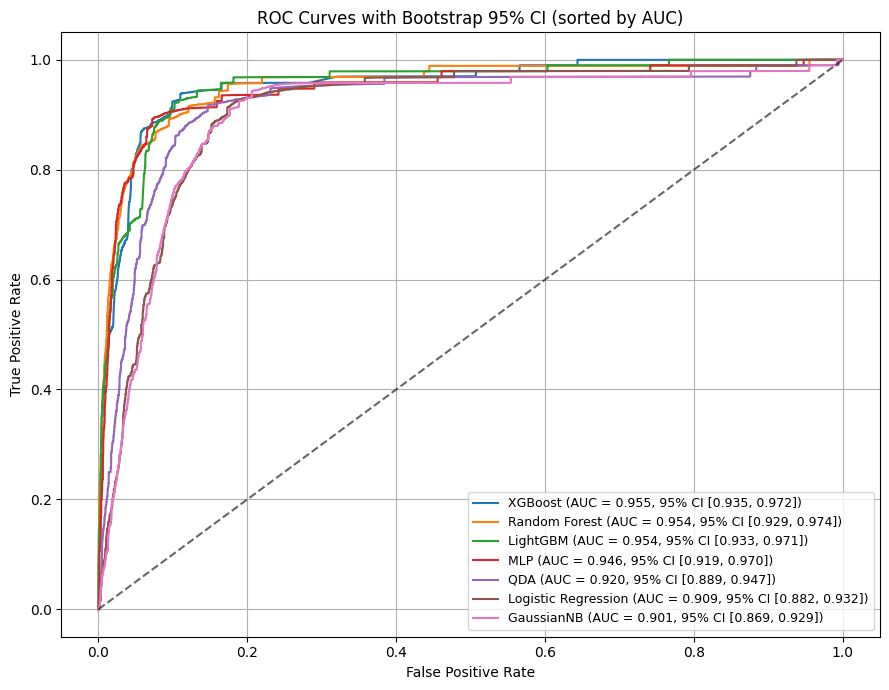
\includegraphics[width=0.85\columnwidth]{Figures/roc_curves.png}
    \caption{ROC curves for the classifiers evaluated using OOF predictions from 5-fold stratified cross-validation.} 
    \label{fig:roc_curves}
\end{figure}

 
\begin{table}[t]
\centering
\caption{Out-of-fold ROC AUC for each classifier, with $95\%$
confidence intervals from $1000$ stratified bootstrap resamples.}
\label{tab:auc_results}
\begin{tabular}{l c}
\hline
\textbf{Classifier} & \textbf{ROC AUC ($95\%$ CI)} \\
\hline
XGBoost              & $0.955$ $[0.935,\,0.972]$ \\
Random Forest        & $0.954$ $[0.929,\,0.974]$ \\
LightGBM             & $0.954$ $[0.933,\,0.971]$ \\
MLP                  & $0.946$ $[0.919,\,0.970]$ \\
QDA                  & $0.920$ $[0.889,\,0.947]$ \\
Logistic Regression  & $0.909$ $[0.882,\,0.932]$ \\
GaussianNB           & $0.901$ $[0.869,\,0.929]$ \\
\hline
\end{tabular}
\end{table}
 
The four ensemble or non-linear methods, XGBoost, LightGBM,
Random Forest, and the MLP, cluster within $\sim 0.01$ AUC of
each other at the top of the ranking, while the two generative
classifiers (QDA, GaussianNB) and the linear classifier
(Logistic Regression) form a second, lower-AUC group separated
by approximately $0.04$ from the leading models. This split is
the first quantitative indication that the discriminating
information in the $20$-feature set is not contained in the
class-conditional means and (co)variances alone, but is in
substantial part carried by higher-order, non-linear
correlations among the features.


\section{Signal Significance on Monte Carlo}
The signal significance $Z$ quantifies how unlikely the observed signal yield would be if the data contained only background. For a counting experiment with expected signal $S$, expected background $B$, and an assumed fractional systematic uncertainty $k$ on $B$,

\begin{equation}
Z =
\frac{S}{\sqrt{B + (kB)^2}}
\label{eq:significance}
\end{equation}

with $k = 0.30$, corresponding to a conservative 30\% systematic uncertainty that absorbs into a single number the smaller individual contributions from theoretical cross-sections, parton-distribution functions, jet-energy scale, lepton efficiencies, and pile-up modelling.The quantities $S$ and $B$ are obtained by summing the per-event luminosity weights over events passing the classifier-score threshold and falling within the signal-region window 
\[
m_{4\ell} \in [110,135)\,\mathrm{GeV}.
\]
The corresponding statistical uncertainties are

\begin{equation}
\sigma_S = \sqrt{\sum_i w_i^2},
\qquad
\sigma_B = \sqrt{\sum_i w_i^2},
\label{eq:yield_uncertainties}
\end{equation}

evaluated separately over the signal and background events\cite{atlas2018higgsmass}. Propagating these uncertainties through Eq.~\ref{eq:significance} yields

\begin{equation}
\sigma_Z^2 =
\frac{\sigma_S^2}{D}
+
\frac{
S^2 (1 + 2k^2B)^2 \sigma_B^2
}{
4D^3
},
\qquad
D = B + (kB)^2,
\label{eq:significance_uncertainty}
\end{equation}

and the corresponding one-sided $p$-value is obtained from

\begin{equation}
p = 1 - \Phi(Z),
\label{eq:pvalue}
\end{equation}

where $\Phi(Z)$ is the cumulative distribution function of the standard normal distribution. In this section, $S$ and $B$ are taken from the Monte Carlo simulation.


\subsection{Score distributions and choice of threshold}
Each classifier outputs a per-event probability score in the interval $[0,1]$; converting this into a binary decision requires a threshold. The optimal value depends on the shape of the classifier score distribution, specifically on how well it separates the signal score distribution from the background score distribution.

Figure~\ref{fig:score_distributions} shows the out-of-fold (OOF) score distributions for signal and background events, normalised separately to unit area, for all seven classifiers. The well-performing classifiers, such as XGBoost, LightGBM, the MLP, Random Forest, and Logistic Regression, produce score distributions in which signal events accumulate near 1 while background events accumulate near 0, with the two distributions clearly separated over a wide score range. QDA and GaussianNB, by contrast, produce signal and background distributions that overlap heavily across most of the score range, with no region in which a clean signal-rich subset can be isolated.

\begin{figure}[htbp]
    \centering
    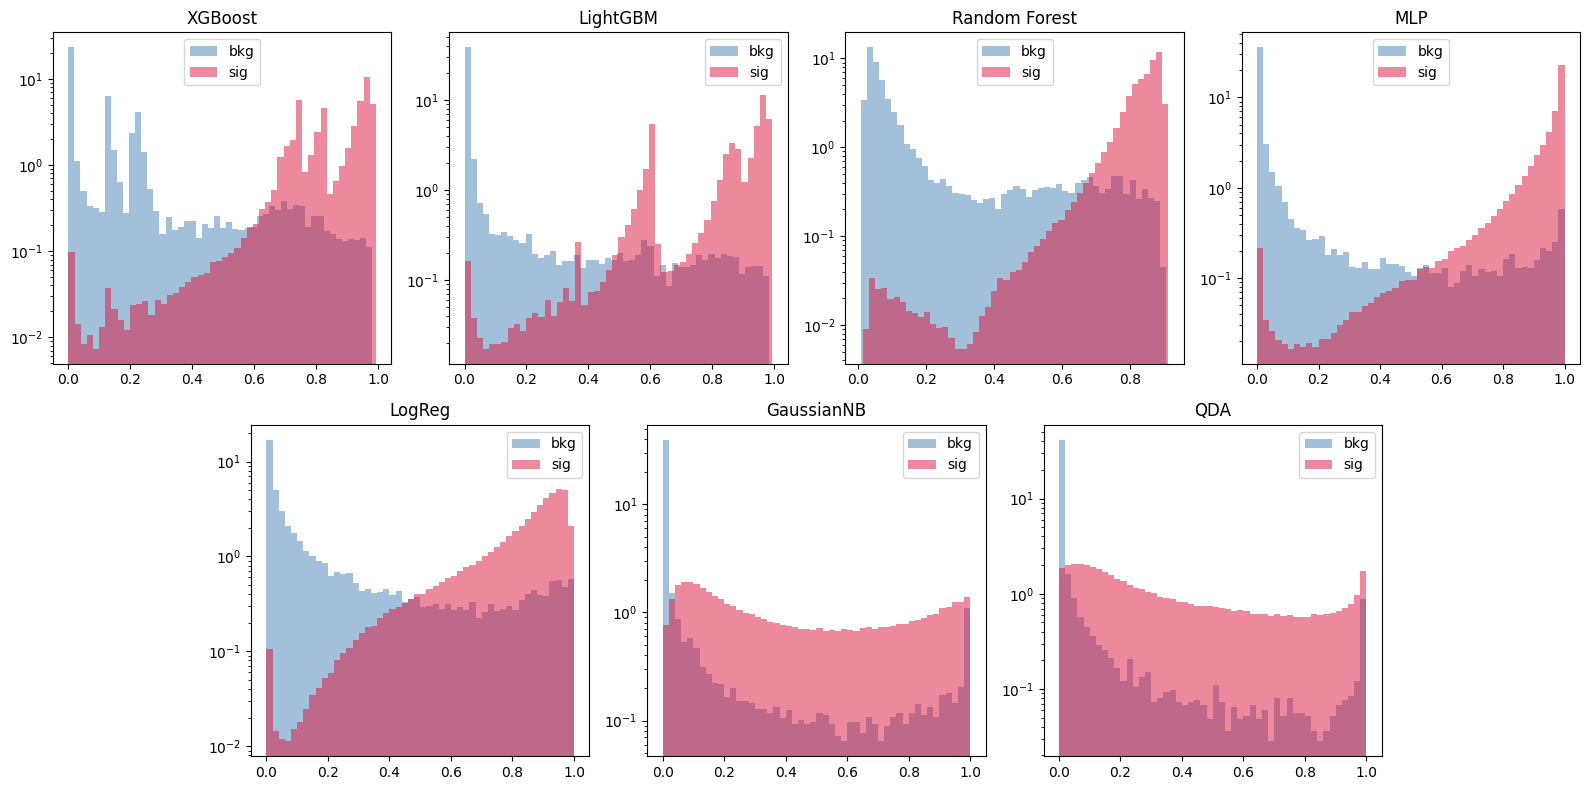
\includegraphics[width=0.90\columnwidth]{Figures/score_distributions.png}
    \caption{Out-of-fold classifier score distributions for signal and background.}
    \label{fig:score_distributions}
\end{figure}

A uniform working point of
\[
\mathrm{threshold} > 0.65
\]
is adopted for all classifiers. For each well-performing classifier, this value lies in the region of low background density and substantial signal density, retaining a large fraction of the signal while suppressing most of the background.

The threshold is further validated through a scan from 0.10 to 0.95 in steps of 0.05, computing $S$, $B$, and $Z$ via Eqs.~\ref{eq:significance}--\ref{eq:significance_uncertainty} on the Monte Carlo OOF scores within the signal-region window. The scan confirms that 0.65 lies within a broad plateau of near-maximal significance $Z$ for the well-performing classifiers, indicating that small variations in the threshold do not significantly degrade the result.

The threshold is further validated through a scan from 0.10 to 0.95 in steps of 0.05, computing SS
S, BB
B, and ZZ
Z via Eqs.~\ref{eq:significance}--\ref{eq:significance_uncertainty} on the Monte Carlo OOF scores within the signal-region window. The scan confirms that 0.65 lies within a broad plateau of near-maximal significance ZZ
Z for the well-performing classifiers, indicating that small variations in the threshold do not significantly degrade the result. The working point is taken at the lower edge of the plateau rather than at its peak, in order to retain enough surviving signal events. Fig.~\ref{fig:xgb_threshold_scan} shows the scan for XGBoost as a representative example; the corresponding scans for the other classifiers exhibit the same behaviour and are reported in appendices.

\begin{figure}[htbp]
\centering
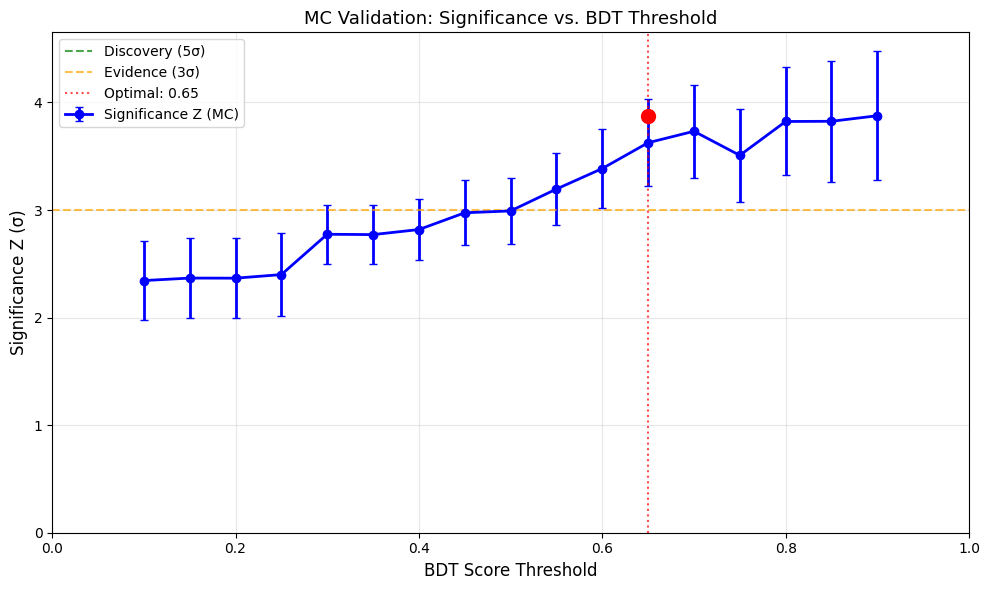
\includegraphics[width=\linewidth]{Figures/xgb_threshold_scan.png}
\caption{XGBoost threshold scan showing the variation of the significance.}
\label{fig:xgb_threshold_scan}
\end{figure}

\subsection{Accuracy and the signal-efficiency–background-rejection balance}
A common temptation is to evaluate classifiers by their raw accuracy, but in this analysis accuracy is misleading. Because the dataset is dominated by background, a classifier that aggressively labels almost every event as background will achieve a very high accuracy while discarding most of the signal. What matters instead is the simultaneous achievement of high signal efficiency and high background rejection. Table~\ref{tab:classifier_performance} lists these three quantities at the $\mathrm{score}>0.65$ working point.

\begin{table}[htbp]
\centering
\small
\caption{Classifier accuracy, signal efficiency, and background rejection at the $\mathrm{score}>0.65$.}
\label{tab:classifier_performance}

\resizebox{0.4\textwidth}{!}{
\begin{tabular}{l c c c}
\hline
Classifier & Accuracy & Signal Eff. & Bkg Rejection \\
\hline
XGBoost & 0.926 & 87.65\% & 92.71\% \\
LightGBM & 0.944 & 70.97\% & 94.96\% \\
Random Forest & 0.909 & 88.16\% & 90.92\% \\
MLP & 0.943 & 84.39\% & 94.58\% \\
Logistic Regression & 0.881 & 78.68\% & 88.31\% \\
QDA & 0.970 & 19.36\% & 98.95\% \\
GaussianNB & 0.955 & 26.98\% & 97.25\% \\
\hline
\end{tabular}
}
\end{table}

As seen in Table~\ref{tab:classifier_performance} the two highest-accuracy classifiers, the QDA at 0.970 and GaussianNB at 0.955, also exhibit the worst signal efficiencies, retaining only 19\% and 27\% of the true signal, respectively. The remaining five classifiers maintain signal efficiencies above 70\% while achieving background rejections between 88\% and 95\%, indicating that they have learned a genuine decision boundary rather than collapsing onto the dominant background class.

The score distributions in Fig.~\ref{fig:score_distributions} make the underlying reason visible: for the five well-performing classifiers, the signal histograms retain substantial density above the 0.65 threshold while the background histograms have already fallen off sharply. In contrast, QDA and GaussianNB produce strongly overlapping signal and background distributions across the full score range, preventing any threshold from recovering a useful signal-versus-background balance. QDA and GaussianNB are therefore excluded from the remainder of the analysis.

\section*{Results}

\section{Signal Significance Evaluation on Monte Carlo}

Applying a classifier threshold of $0.65$ for each of the five retained classifiers, the corresponding signal significances are evaluated in the signal-region window $m_{4\ell} \in [110, 135)$~GeV. The no-ML baseline, computed on the same Monte Carlo events without any classifier selection, is also evaluated for comparison. The results are summarized in Table~\ref{tab:mc_significance} and visualized in the forest plot of Fig.~\ref{fig:significance_forest}.

\begin{table}[h]
\centering
\caption{Monte Carlo signal significance at threshold $>0.65$ in the window $m_{4\ell} \in [110, 135)$~GeV. The no-ML baseline applies only the mass-window selection.}
\label{tab:mc_significance}
\begin{tabular}{l c}
\hline
\textbf{Method} & $Z$ ($\sigma$) \\
\hline
No ML baseline       & $2.32 \pm 0.36$ \\
XGBoost              & $3.63 \pm 0.40$ \\
Random Forest        & $3.37 \pm 0.36$ \\
LightGBM             & $3.36 \pm 0.40$ \\
Logistic Regression  & $2.95 \pm 0.33$ \\
MLP                  & $2.47 \pm 0.42$ \\
\hline
\end{tabular}
\end{table}

\begin{figure}[htbp]
    \centering
    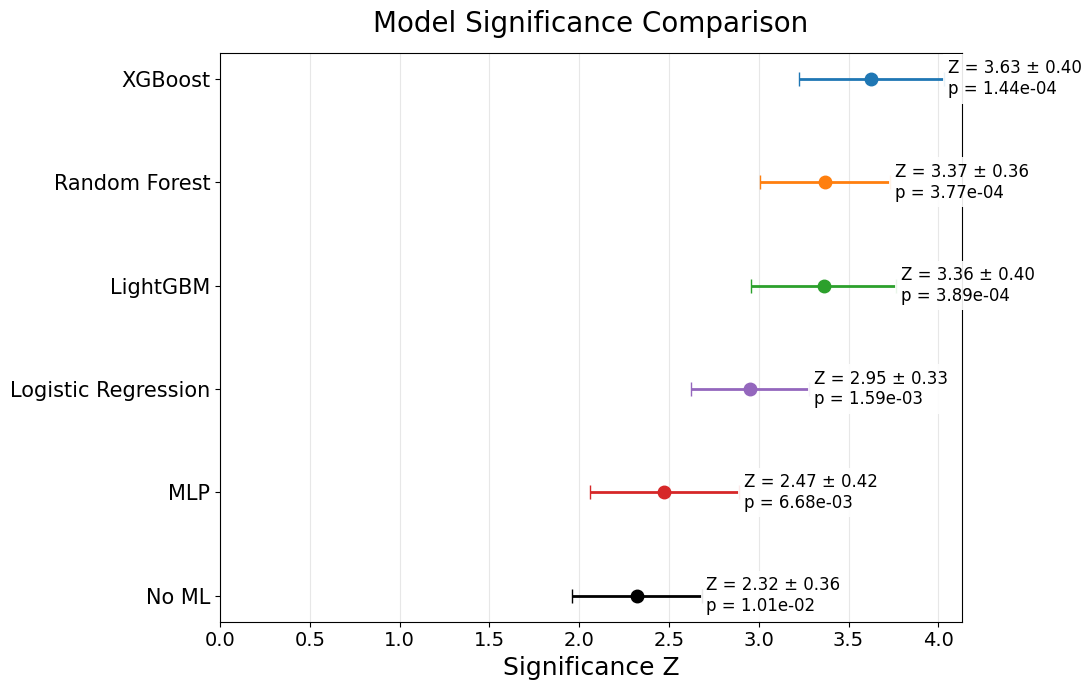
\includegraphics[width=0.85\columnwidth]{Figures/significance_forest.png}
    \caption{Signal significance comparison for the five classifiers on Monte Carlo.}
    \label{fig:significance_forest}
\end{figure}


XGBoost is the most sensitive of the five retained classifiers on Monte Carlo, with Random Forest and LightGBM following within their uncertainties. All five ML-based selections improve upon the no-ML baseline significance of $2.32 \pm 0.36$, with the boosted-tree and Random Forest models providing the largest gains, an improvement factor of approximately $1.6\times$.



\section{Application to Real ATLAS Data}

The five retained classifiers are applied to the 1,279 real ATLAS events. Each event is scored independently using the five fold-models from the 5-fold cross-validation, and the resulting scores are averaged to obtain the final event-level classifier score. Events are selected if their averaged score exceeds the working point of $0.65$ and their four-lepton invariant mass falls within the signal-region window $m_{4\ell} \in [110, 135)$~GeV.

To compute the signal significance, the expected background in the signal region is estimated using two independent methods. The first is the Monte Carlo prediction, in which $B$ is taken directly from the simulated background yield surviving both the classifier cut and the mass-window selection. The second is a data-driven sideband extrapolation, in which $B$ is estimated entirely from data: events passing the classifier cut in the sidebands $m_{4\ell} \in [90, 105)$~GeV and $[140, 155)$~GeV are counted and scaled by the ratio of signal-region width to total sideband width, under the assumption of a locally smooth background. The two methods make nearly orthogonal assumptions, so their agreement serves as an internal cross-check of the result.

The signal yield is defined as $S = N_{\text{obs}} - B$, and is then propagated through Eqs.~\ref{eq:significance}--\ref{eq:significance_uncertainty} to obtain $Z$ and $\sigma_Z$.

An additional no-ML baseline is also computed on the real data, applying only the mass-window selection with no classifier cut. This baseline gives $Z = 3.42 \pm 0.92\,\sigma$ on the real data, and is the reference against which the classifier-based selections are compared. The results for all five retained classifiers, together with the no-ML baseline, are summarized in Table~\ref{tab:realdata_significance} and visualized in the forest plot of Figures~\ref{fig:z_combined}.


\begin{table}[!t]
\centering
\caption{Real-data signal significance for each retained classifier, under the Monte Carlo prediction and the data-driven sideband-extrapolation methods. The no-ML row uses only the mass-window selection ($m_{4\ell} \in [110, 135)$~GeV) with no classifier cut.}
\label{tab:realdata_significance}
\renewcommand{\arraystretch}{1.2}
\setlength{\tabcolsep}{4pt}
\footnotesize
\begin{tabular}{lcccc}
\hline
\textbf{Classifier} & \multicolumn{2}{c}{\textbf{MC prediction}} & \multicolumn{2}{c}{\textbf{Sideband}} \\
                    & $B$   & $Z$              & $B$   & $Z$ \\
\hline
No ML (baseline)    & 31.95 & $3.42 \pm 0.92$ & 31.95 & $3.42 \pm 0.92$ \\
XGBoost             & 17.96 & $4.24 \pm 1.10$ & 16.67 & $4.70 \pm 1.35$ \\
LightGBM            & 15.13 & $4.66 \pm 1.22$ & 14.17 & $5.08 \pm 1.50$ \\
Random Forest       & 21.66 & $3.42 \pm 0.94$ & 23.33 & $3.02 \pm 0.95$ \\
MLP                 & 28.49 & $2.93 \pm 0.90$ & 17.50 & $6.03 \pm 1.55$ \\
Logistic Regression & 19.91 & $3.37 \pm 0.97$ & 35.83 & $0.74 \pm 0.55$ \\
\hline
\end{tabular}
\end{table}


\begin{figure}[htbp]
    \centering
        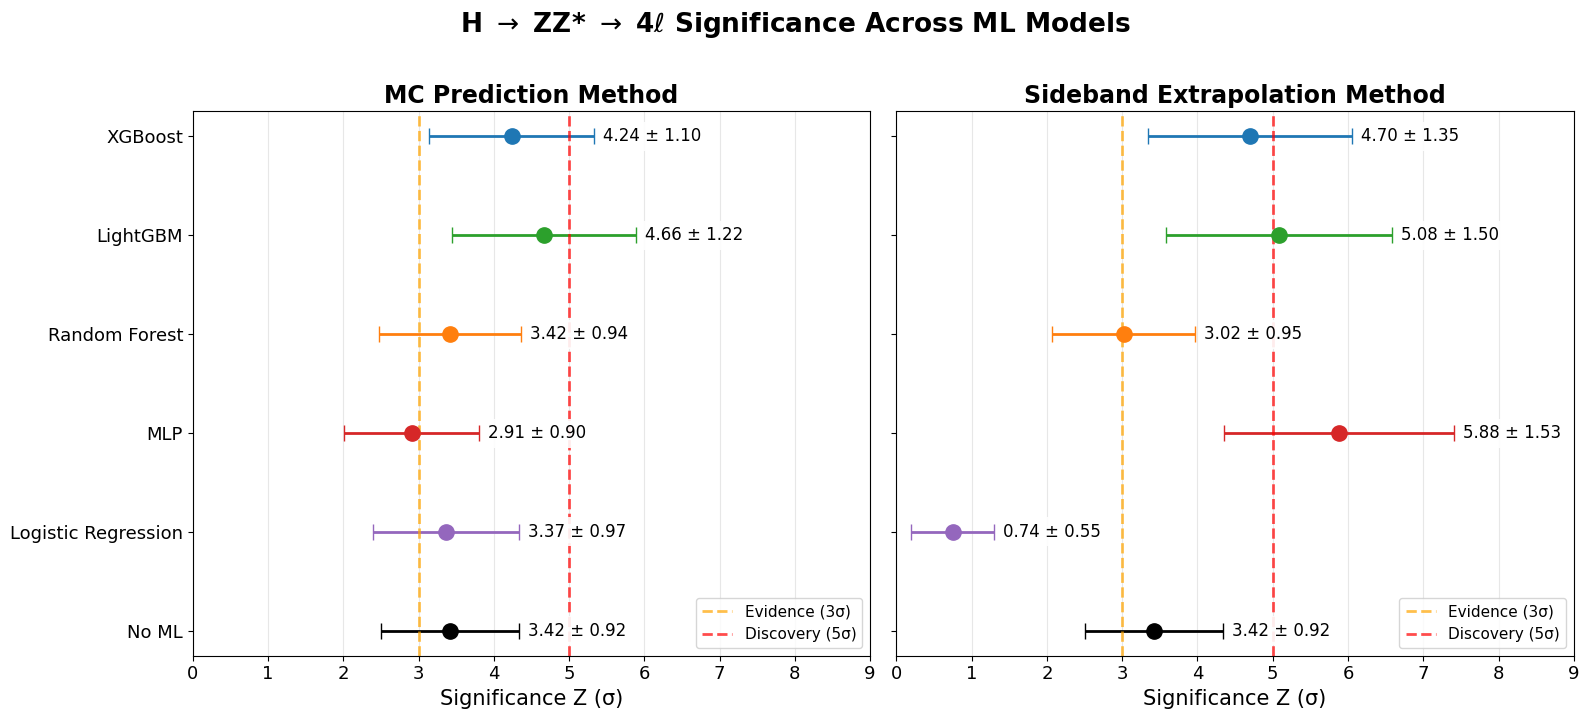
\includegraphics[width=\linewidth]{Figures/z_forest_mc.png}
    \caption{Signal significance $Z$ for under two background estimation methods: (a) Monte Carlo prediction and (b) sideband extrapolation.}
    \label{fig:z_combined}
\end{figure}


\section*{Analysis and Validation}

\subsection*{A. Interpretation of the Monte Carlo Results}

XGBoost is the most sensitive of the five retained classifiers on Monte Carlo, with Random Forest and LightGBM following within their uncertainties. All five ML-based selections improve upon the no-ML baseline significance of $2.32 \pm 0.36$, with the boosted-tree and Random Forest models providing the largest gains, an improvement factor of approximately $1.6\times$. This confirms that on simulation, where signal/background labels are known exactly, every well-performing classifier extracts more sensitivity than the kinematic-cut baseline.

\subsection*{B. Validation Against the No-ML Baseline on Real Data}

The same comparison repeated on the 1,279 real ATLAS events is the central validation of this work, since it is the test of whether the gains seen on simulation transfer to data. Tables~V and~VI together permit a direct MC $\to$ data readout for each classifier. Three patterns are visible:

\textbf{XGBoost and LightGBM.} Both improve on the no-ML baseline of $Z = 3.42 \pm 0.92\,\sigma$ under both background-estimation methods, with central values that agree across the two methods within their uncertainties. The improvement is at the $1$--$1.5\,\sigma$ level in real data, consistent with the $\sim 1.6\times$ factor seen on MC.

\textbf{MLP and Logistic Regression.} Both show large disagreement between the two background-estimation methods. The MLP rises from $Z = 2.93 \pm 0.90$ under the MC prediction to $Z = 6.03 \pm 1.55$ under the sideband extrapolation, while Logistic Regression collapses from $Z = 3.37 \pm 0.97$ to $Z = 0.74 \pm 0.55$. This inconsistency is the diagnostic: neither model's real-data result can be claimed as evidence, because their measured significance depends on which assumption is made about the background. The MLP appears to over-aggressively cut sideband events while Logistic Regression apparently retains too many, but in either direction the disagreement disqualifies the result.

\textbf{Random Forest.} Consistent between the two methods ($Z = 3.42 \pm 0.94$ vs.\ $3.02 \pm 0.95$), but at a lower significance than XGBoost and LightGBM and, on this measurement, indistinguishable from the no-ML baseline. Random Forest is therefore robust but not sensitive enough to claim an improvement over the kinematic-cut analysis on data.


\section*{Discussion and Conlusion}
\subsection{Main Contributions and Key Findings}
This work presents the first standalone machine-learning benchmark for the $H \to ZZ^* \to 4\ell$ channel, comparable in scope to existing standalone Higgs benchmarks on other channels, comparing seven classifier families under a common 5-fold cross-validation protocol on twenty physics-motivated features, and carrying the trained models through to a real-data test on the 1,279 real ATLAS events from the 2025 Open Data release at $\sqrt{s} = 13$~TeV and $36.6~\mathrm{fb}^{-1}$. A two-method validation protocol, Monte Carlo prediction vs.\ data-driven sideband extrapolation, is used to distinguish robust real-data signals from results driven by background-modelling assumptions. The two project objectives, constructing the benchmark and testing real-data generalization, are therefore both met.

Among the seven classifiers tested, XGBoost and LightGBM are the most reliable. Both reach evidence-level significance, with $Z = 4.24 \pm 1.10\,\sigma$ and $Z = 4.66 \pm 1.22\,\sigma$ under the Monte Carlo background prediction, and consistent results under the data-driven sideband method, yielding $Z = 4.70 \pm 1.35\,\sigma$ and $Z = 5.08 \pm 1.50\,\sigma$, respectively. The MLP and Logistic Regression models show large disagreement between the two background-estimation methods, so their results are not robust enough to be claimed as evidence; Random Forest is consistent across methods but does not improve over the no-ML baseline on real data; and GaussianNB and QDA fail to achieve competitive performance and are excluded. The original research question, whether a classifier trained only on simulation can identify the Higgs boson when applied directly to real ATLAS data, is therefore answered in the affirmative.

\textbf{Key finding:} evidence for the Higgs boson is supported by two independent classifiers and validated under two independent background-estimation methods.

\subsection{Limitations and Future Work}
The dominant limitation of the analysis is statistical: per-classifier uncertainties of $\sigma_Z \approx 1$--$1.5\,\sigma$, driven by the limited size of the Open Data sample relative to the full Run-2 dataset of the official ATLAS measurements, mask the differences between the leading classifiers, and the absolute significance values reported here remain a factor of several below the official ATLAS discovery sensitivity in the same channel. Natural extensions of this work include domain-adaptation training that exposes the classifier to control-region real data in addition to simulation, ensembling XGBoost and LightGBM, the two classifiers that pass the cross-method validation, provided their correlations are properly tracked, and extending the benchmark to the off-shell region and to spin-parity discrimination, where the same $4\ell$ topology is used to address physics analyses beyond signal identification.

\section*{Acknowledgment}
We would like to express our sincere gratitude to Dean Reza Malekian of the College of Science and Engineering and Habet Madoyan, Chair of the BSDS Program at AUA, for their continued support throughout the development of this project. This work would not have been possible without the ATLAS Open Data initiative and the broader ATLAS Collaboration.
Artificial-intelligence tools, ChatGPT and Grammarly, were used in the preparation of this paper solely to assist with grammar, spelling, and sentence-level phrasing. All scientific content, methodology, analysis, results, and conclusions are the authors' own work.



% ... last section content ...

\bibliographystyle{IEEEtran}
\bibliography{references}



\clearpage
\section*{Appendix}

% ===================== TABLE =====================
\begin{center}
\captionof{XGBoost hyperparameter grid search.
Mean OOF AUC and per-fold standard deviation across the inner
$5$-fold cross-validation.}
\label{tab:xgb_grid}

\begin{tabular}{c c c}
\hline
\textbf{max\_depth} & \textbf{min\_child\_weight} & \textbf{AUC (mean $\pm$ std)} \\
\hline
3 & 1  & 0.9484 $\pm$ 0.0326 \\
3 & 5  & 0.9530 $\pm$ 0.0229 \\
3 & 10 & 0.9471 $\pm$ 0.0297 \\
\textbf{4} & \textbf{1}  & \textbf{0.9616 $\pm$ 0.0254} \\
4 & 5  & 0.9518 $\pm$ 0.0211 \\
4 & 10 & 0.9468 $\pm$ 0.0254 \\
5 & 1  & 0.9563 $\pm$ 0.0219 \\
5 & 5  & 0.9587 $\pm$ 0.0143 \\
5 & 10 & 0.9516 $\pm$ 0.0278 \\
\hline
\end{tabular}
\end{center}

\vspace{0.6cm}

% ===================== TSCAN FIGURE =====================
\begin{center}
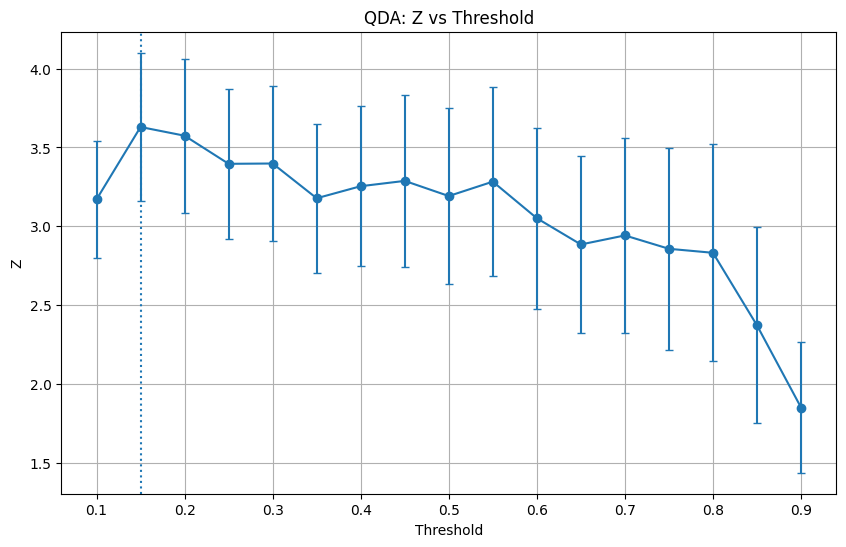
\includegraphics[width=0.31\textwidth]{Figures/tscan1}
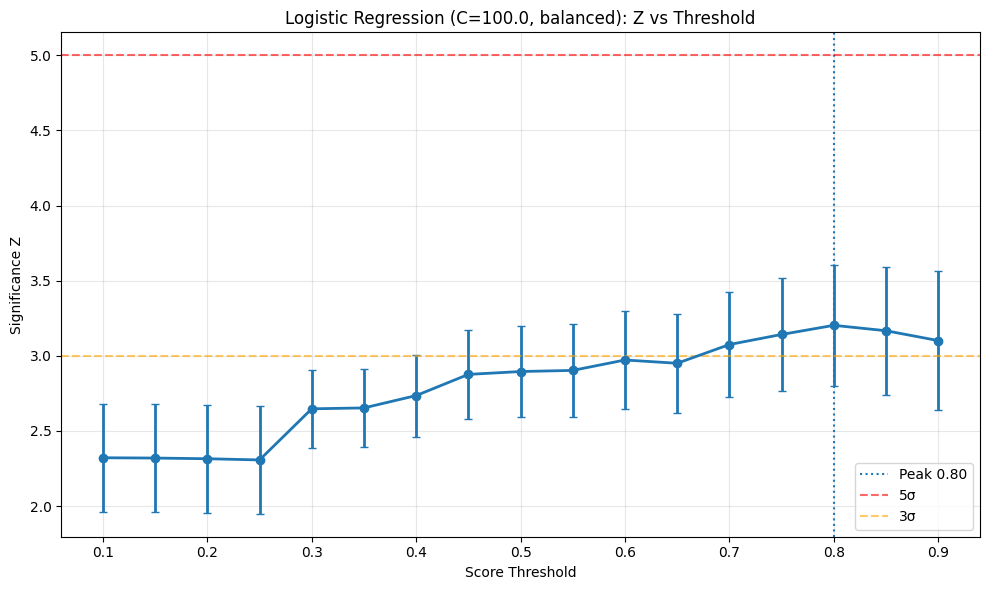
\includegraphics[width=0.31\textwidth]{Figures/tscan2}
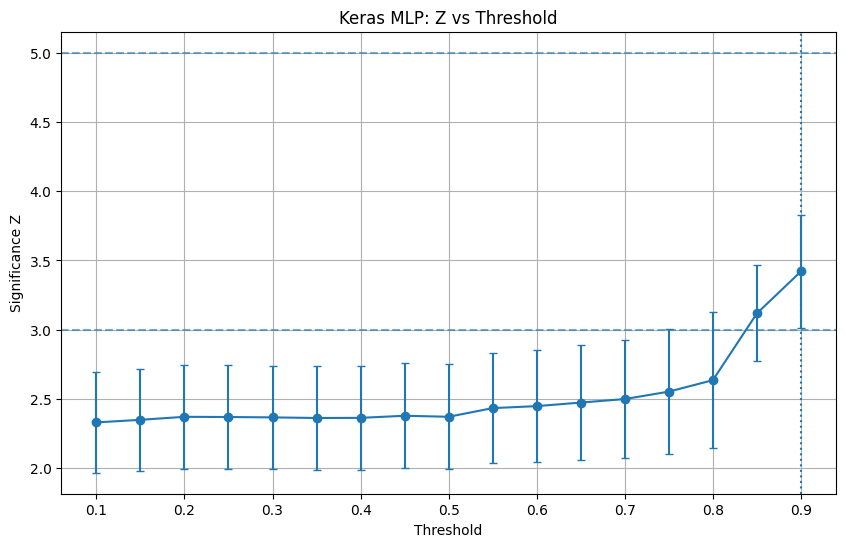
\includegraphics[width=0.31\textwidth]{Figures/tscan3}

\vspace{0.2cm}

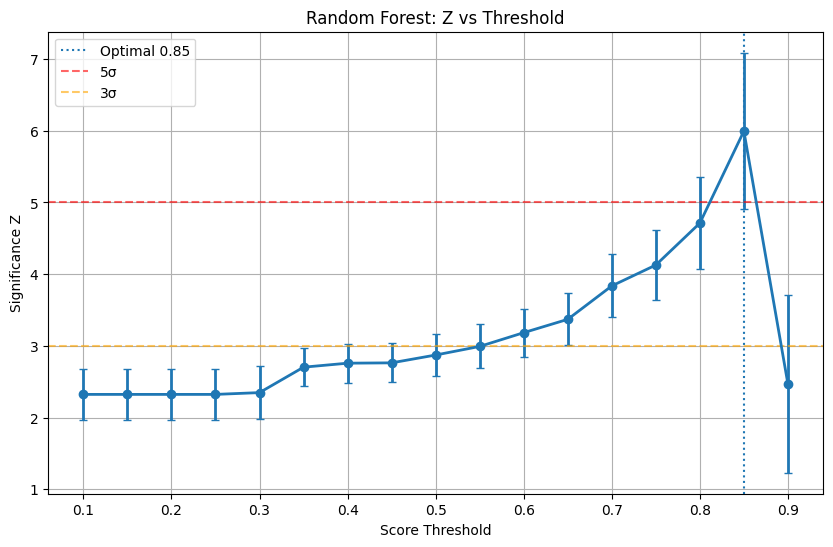
\includegraphics[width=0.31\textwidth]{Figures/tscan4}
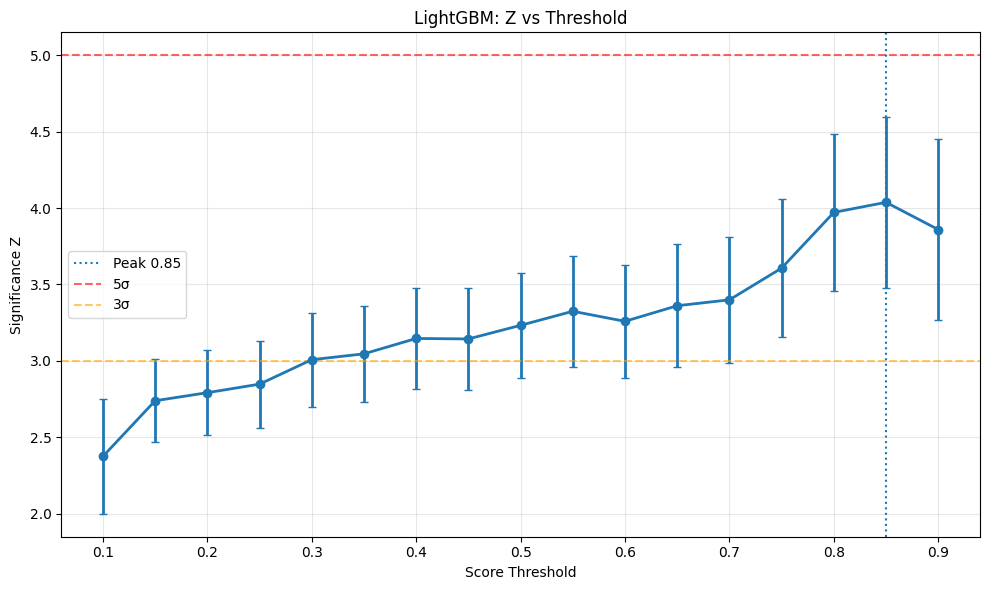
\includegraphics[width=0.31\textwidth]{Figures/tscan5}
\includegraphics[width=0.31\textwidth]{Figures/tscan6}

\captionof{Threshold scan of ML models}
\label{fig:threshold_scan}
\end{center}

\clearpage




\resizebox{\textwidth}{!}{%}
\begin{minipage}{1.35\textwidth}

% Row 1
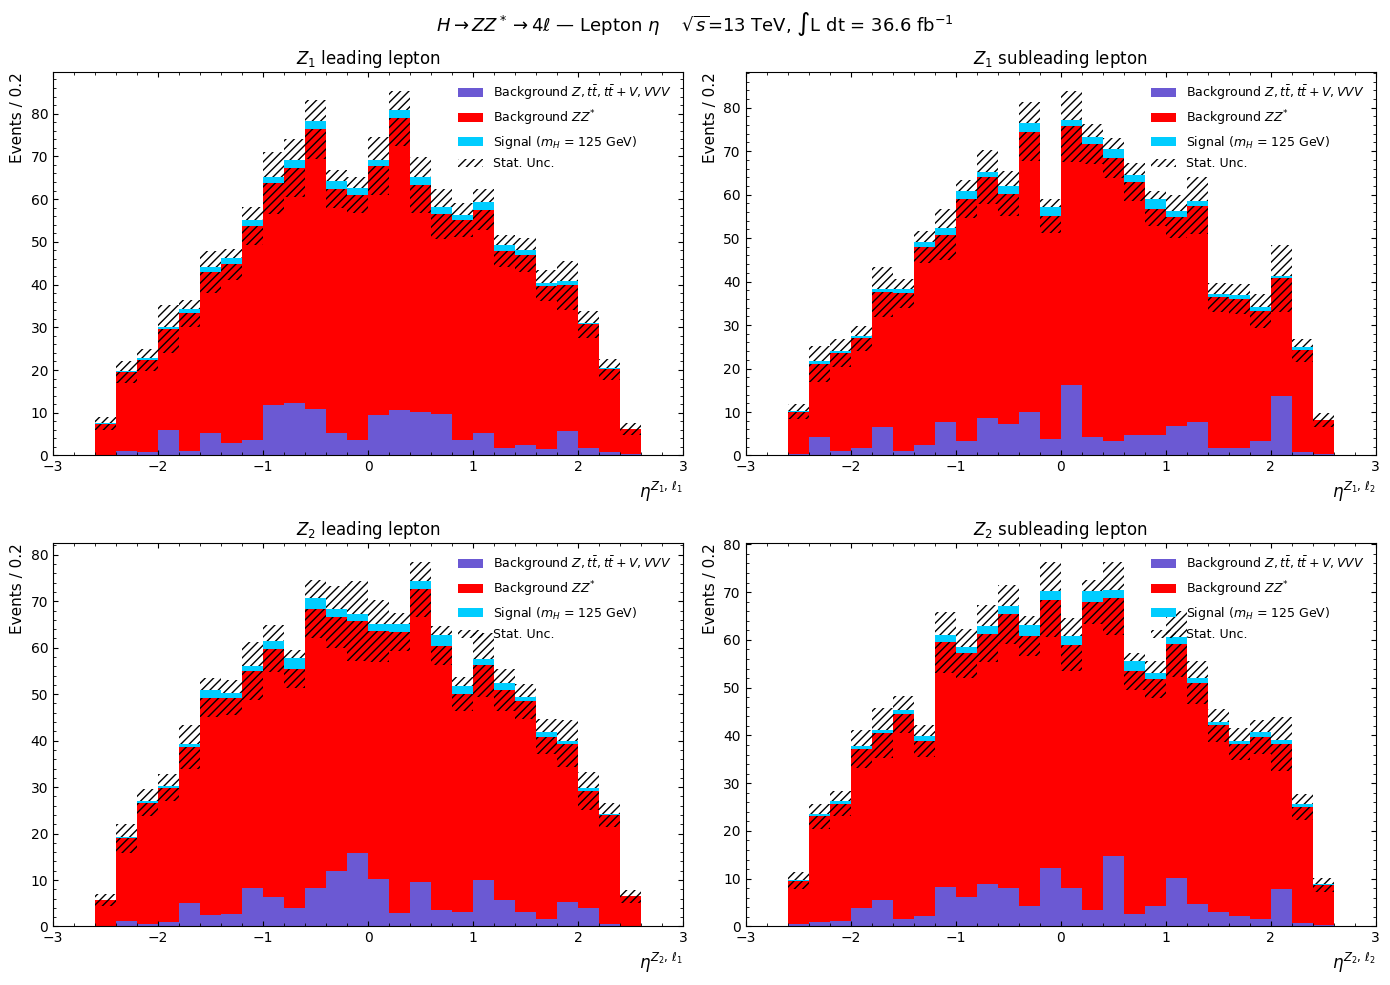
\includegraphics[width=0.28\textwidth]{Figures/download (4).png}\hfill
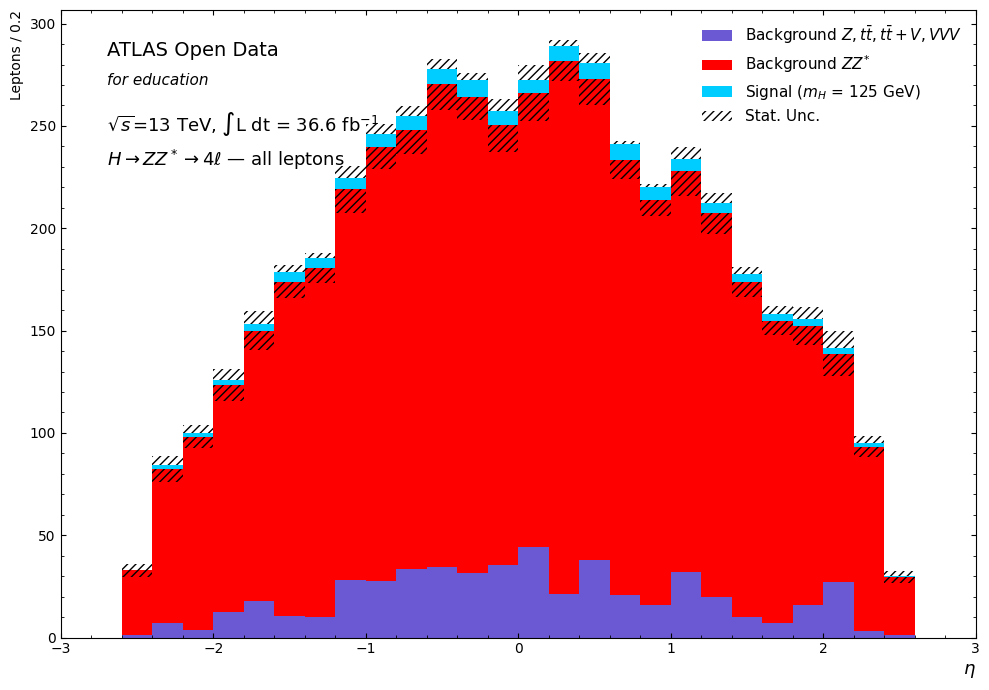
\includegraphics[width=0.28\textwidth]{Figures/download (5).png}\hfill
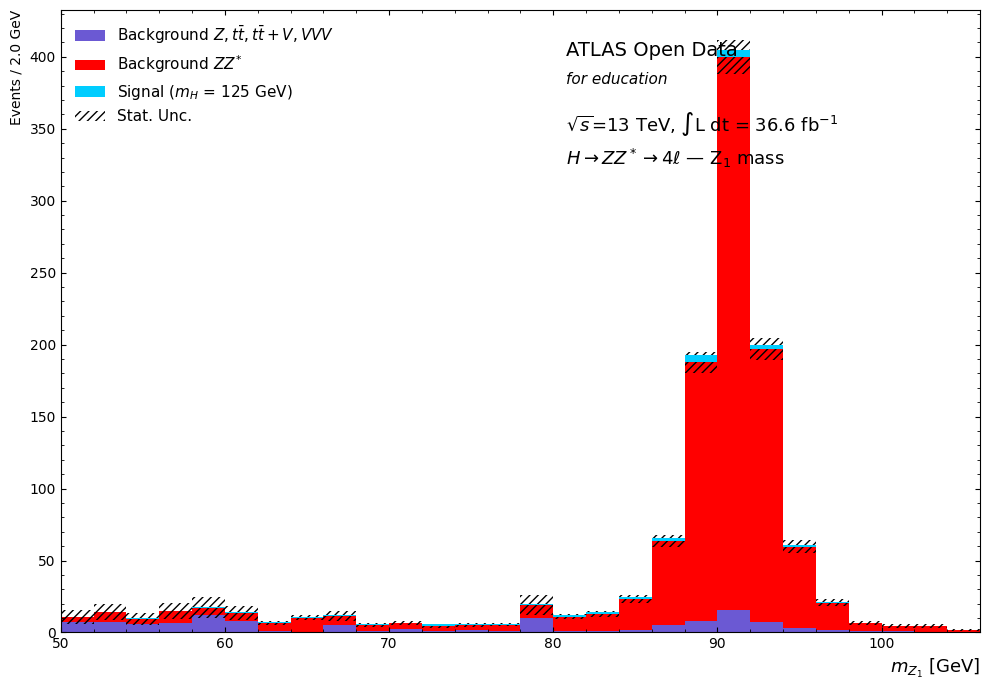
\includegraphics[width=0.28\textwidth]{Figures/download (6).png}

\vspace{0.3cm}

% Row 2
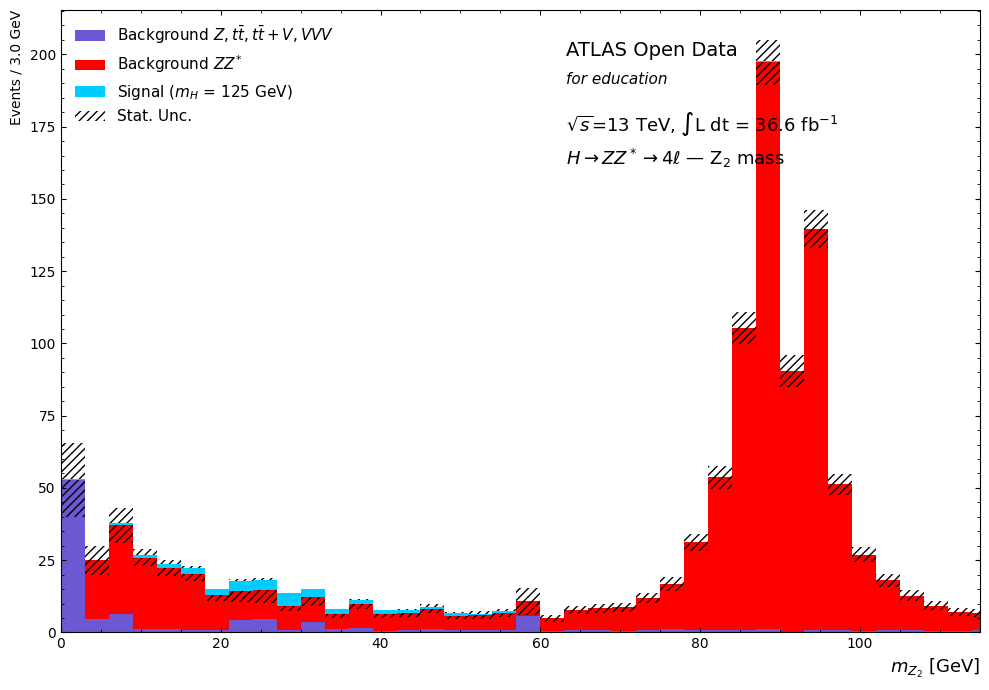
\includegraphics[width=0.28\textwidth]{Figures/download (7).png}\hfill
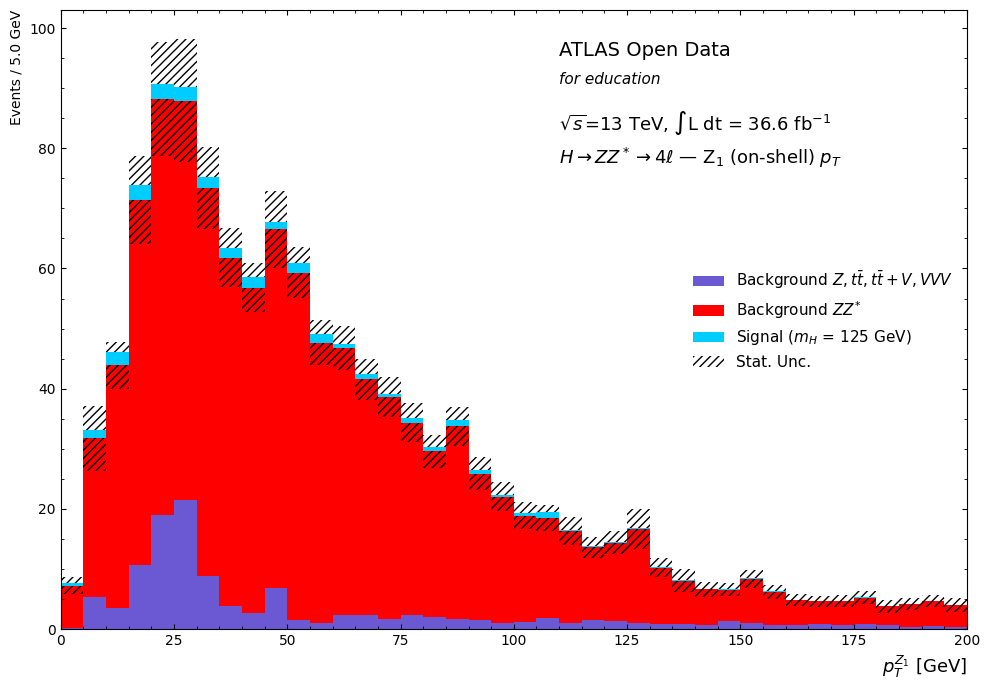
\includegraphics[width=0.28\textwidth]{Figures/download (8).png}\hfill
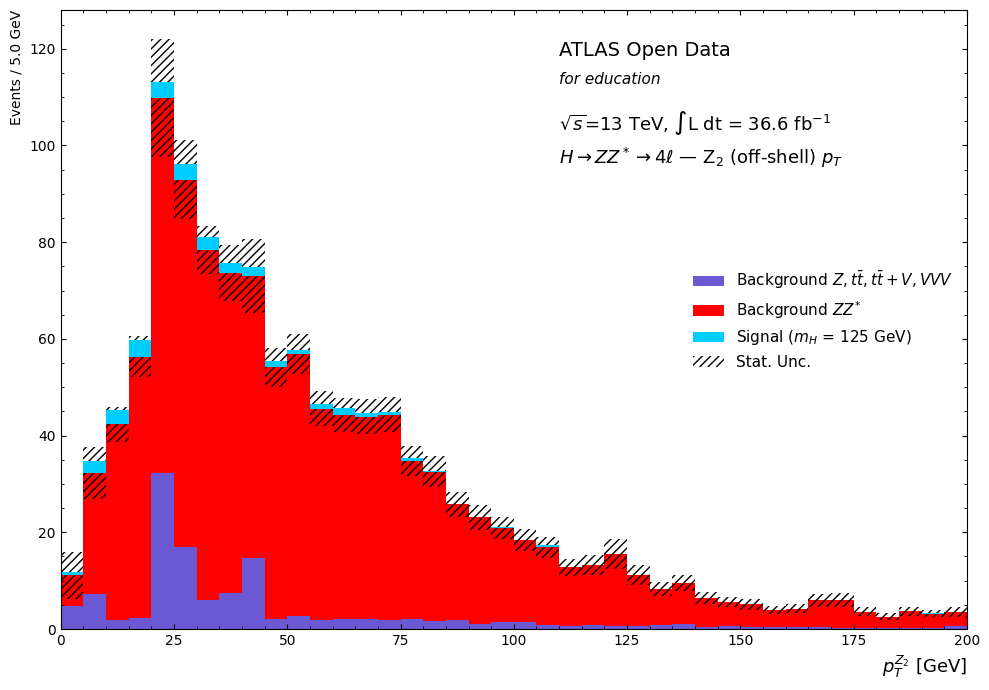
\includegraphics[width=0.28\textwidth]{Figures/download (9).png}

\vspace{0.3cm}

% Row 3
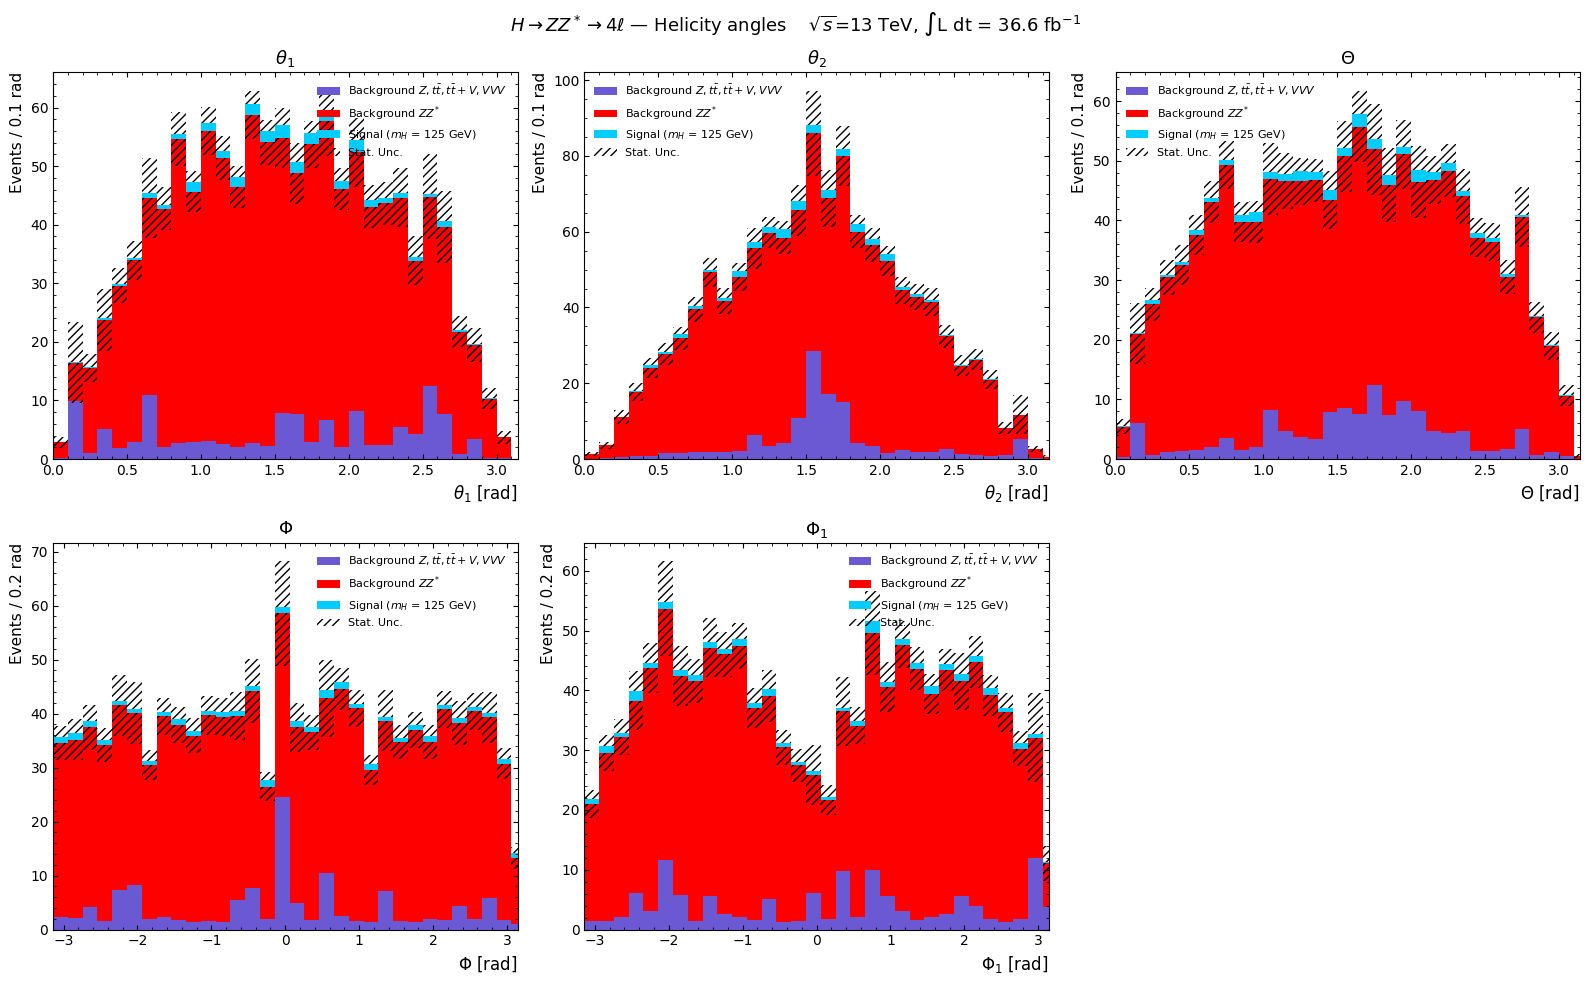
\includegraphics[width=0.28\textwidth]{Figures/download (10).png}\hfill
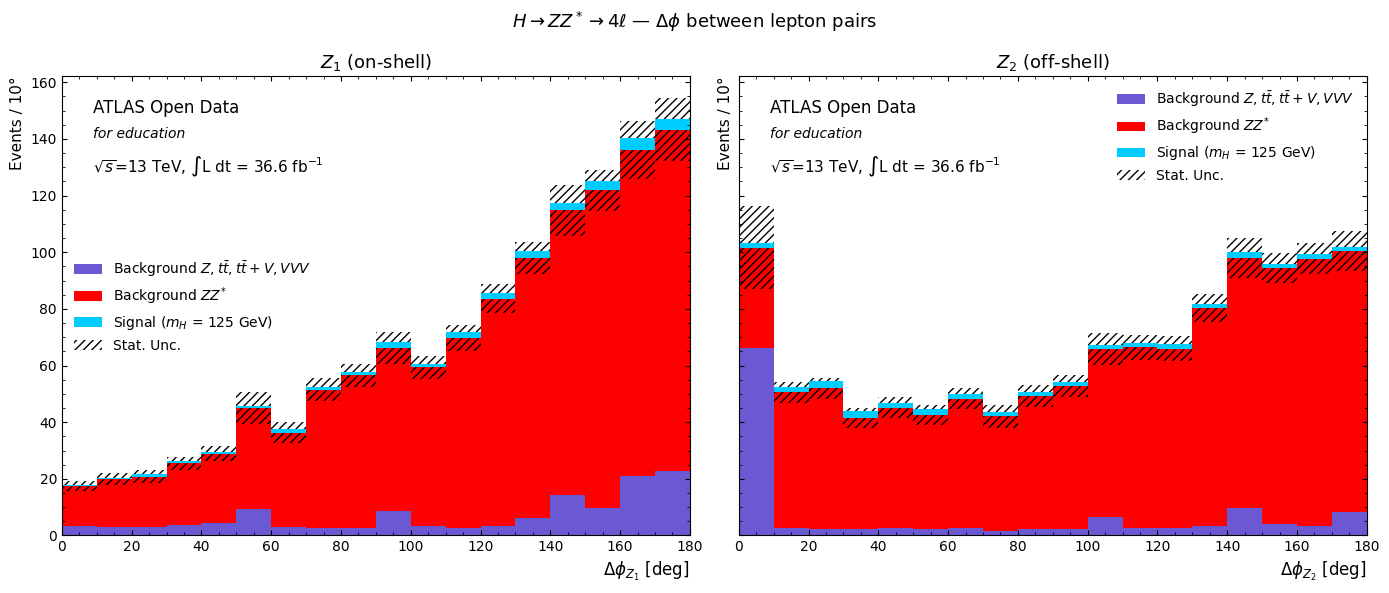
\includegraphics[width=0.28\textwidth]{Figures/download (11).png}\hfill
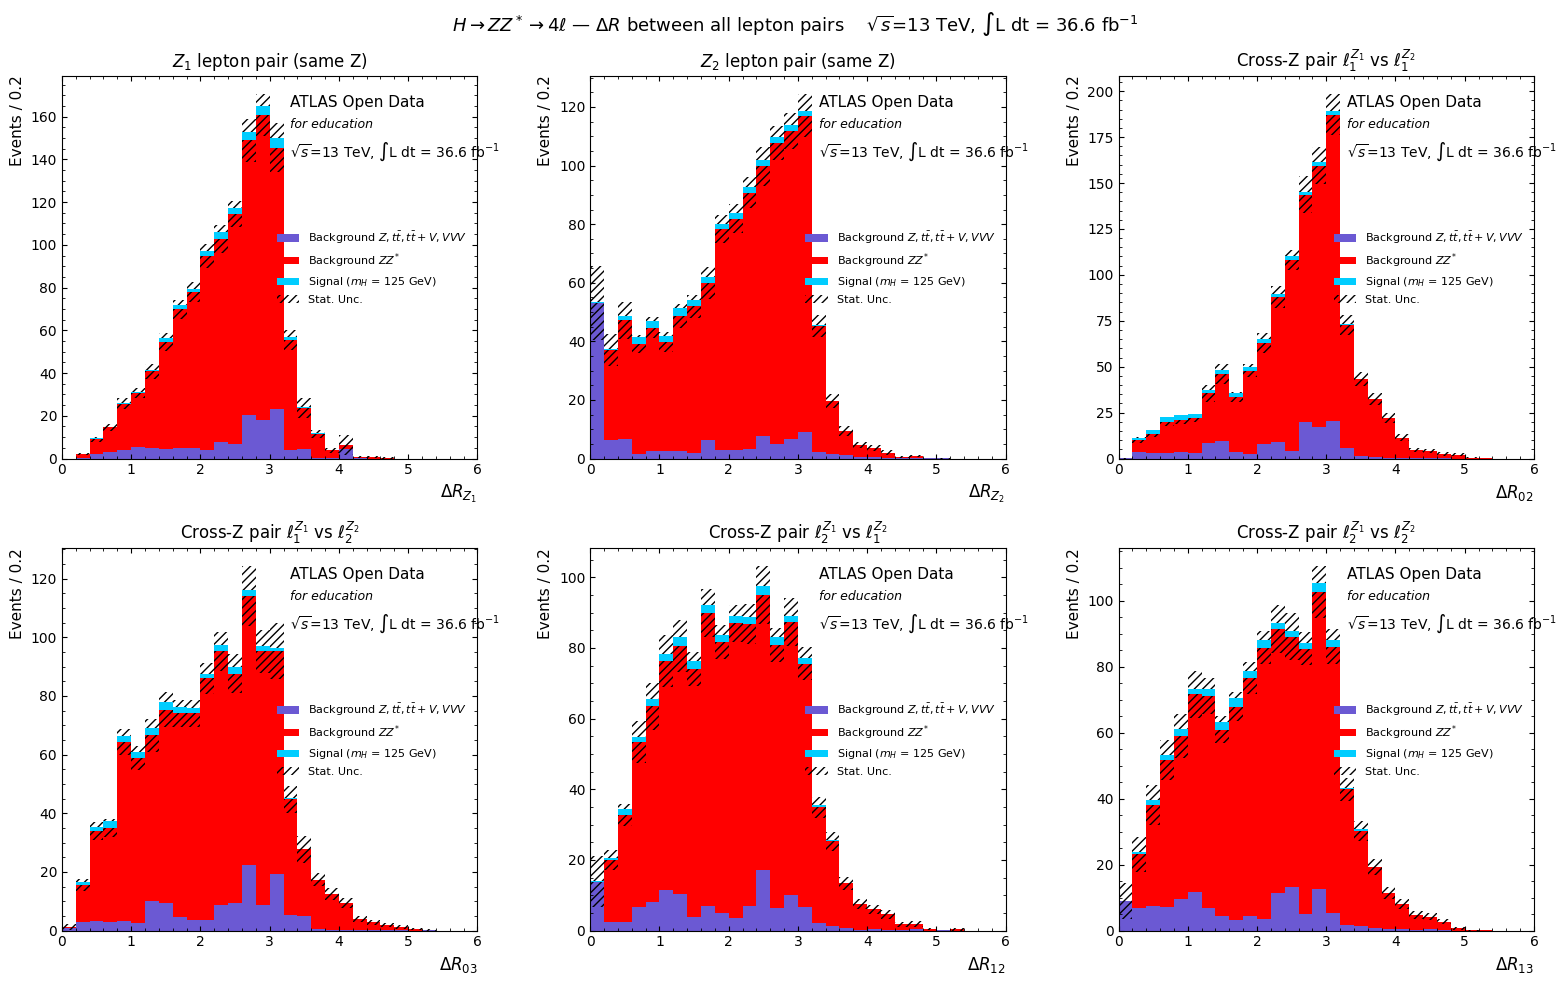
\includegraphics[width=0.28\textwidth]{Figures/download (12).png}

\vspace{0.3cm}

% Row 4
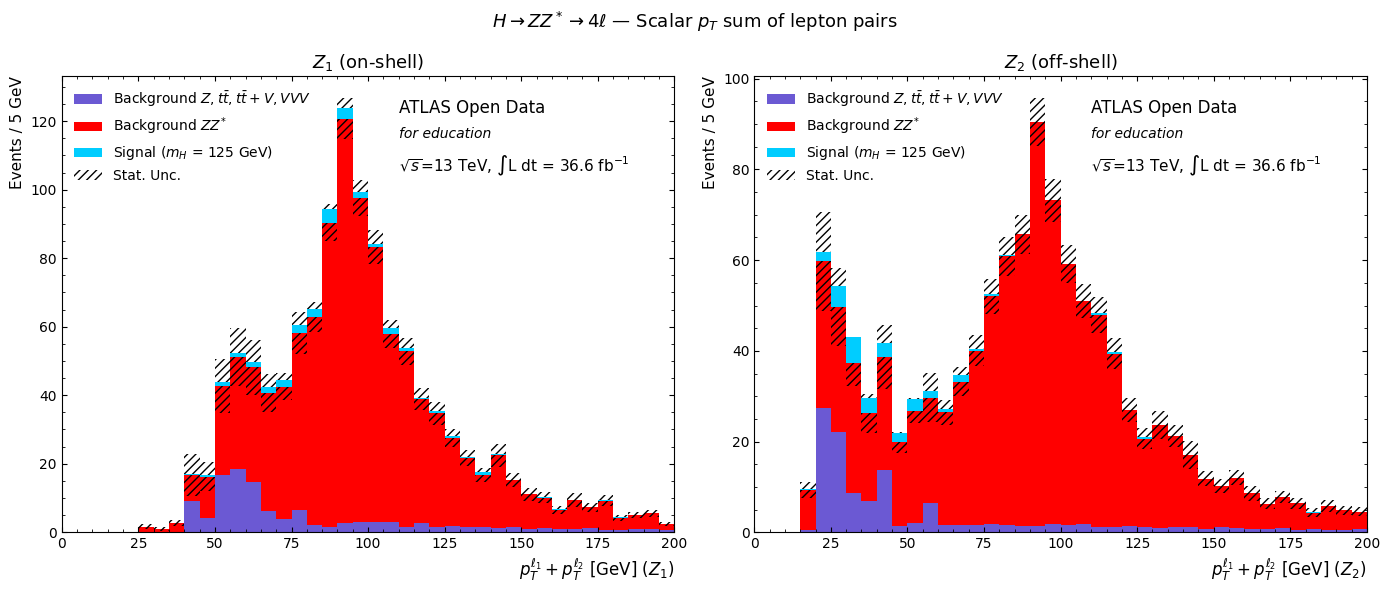
\includegraphics[width=0.28\textwidth]{Figures/download (13).png}\hfill
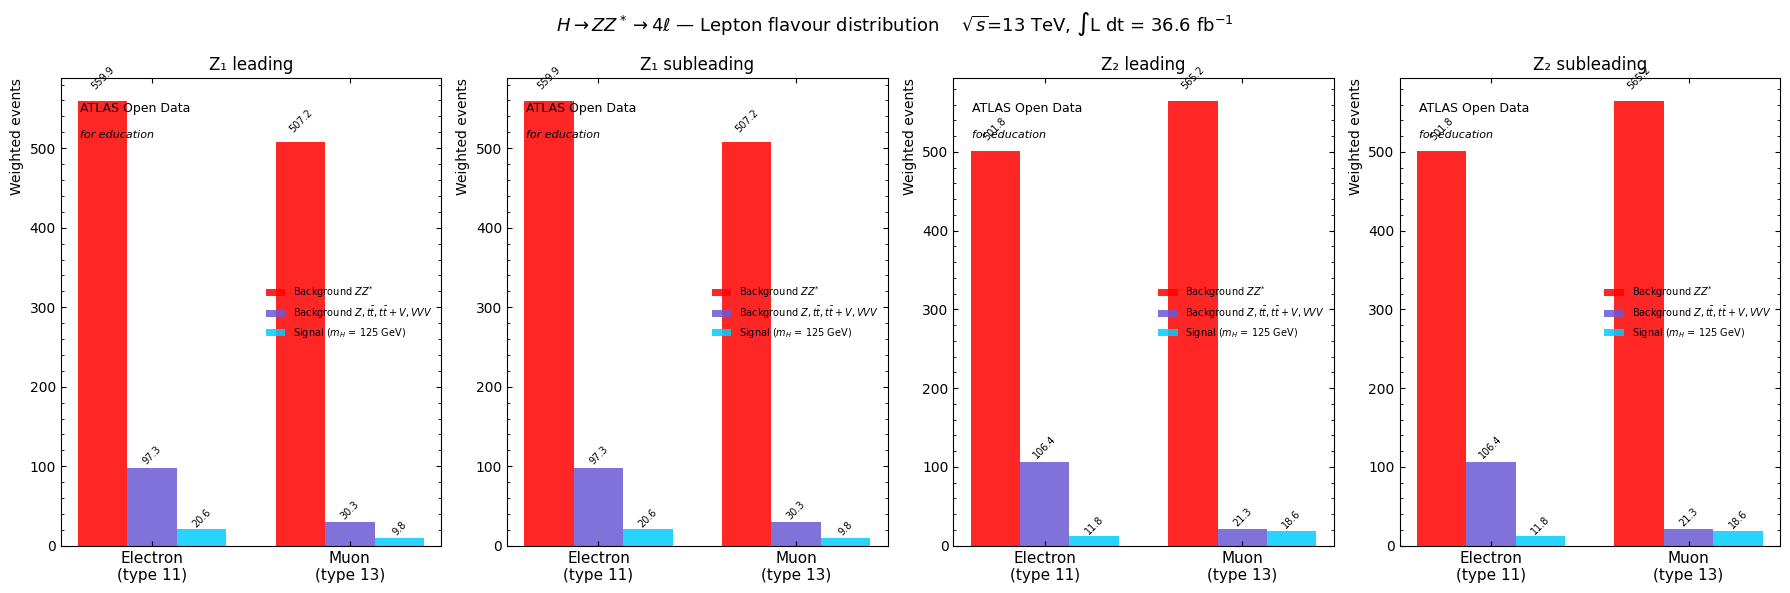
\includegraphics[width=0.28\textwidth]{Figures/download (14).png}\hfill
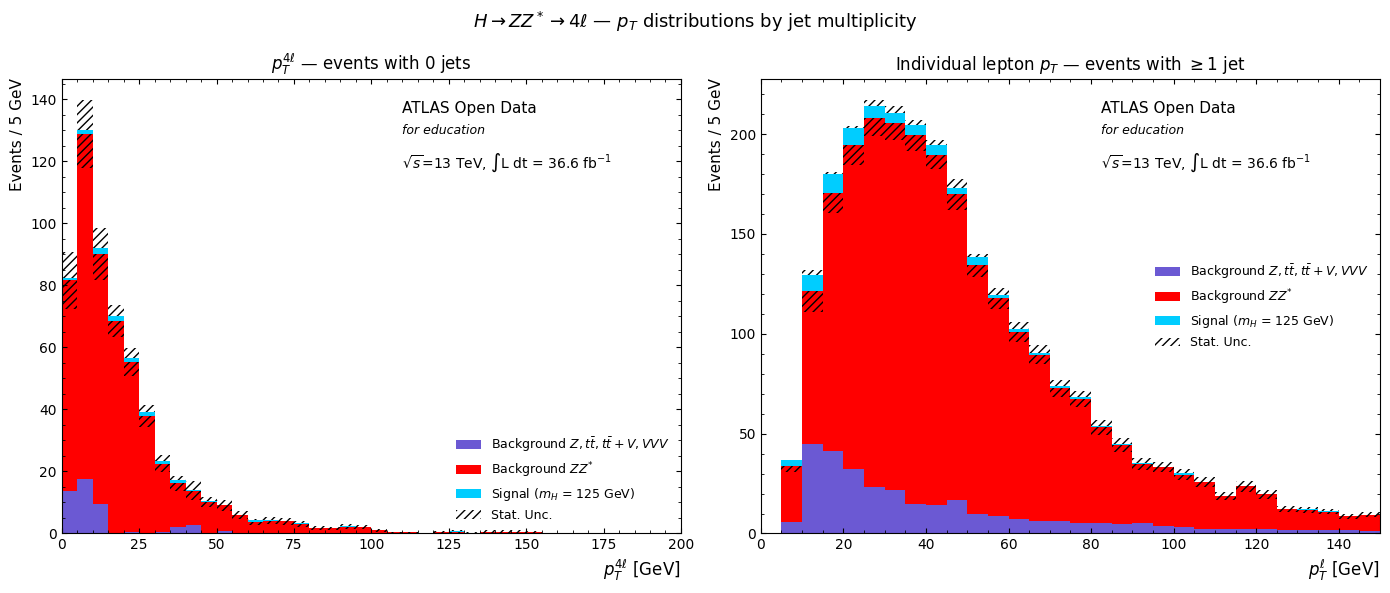
\includegraphics[width=0.28\textwidth]{Figures/download (15).png}

\vspace{0.3cm}

% Row 5
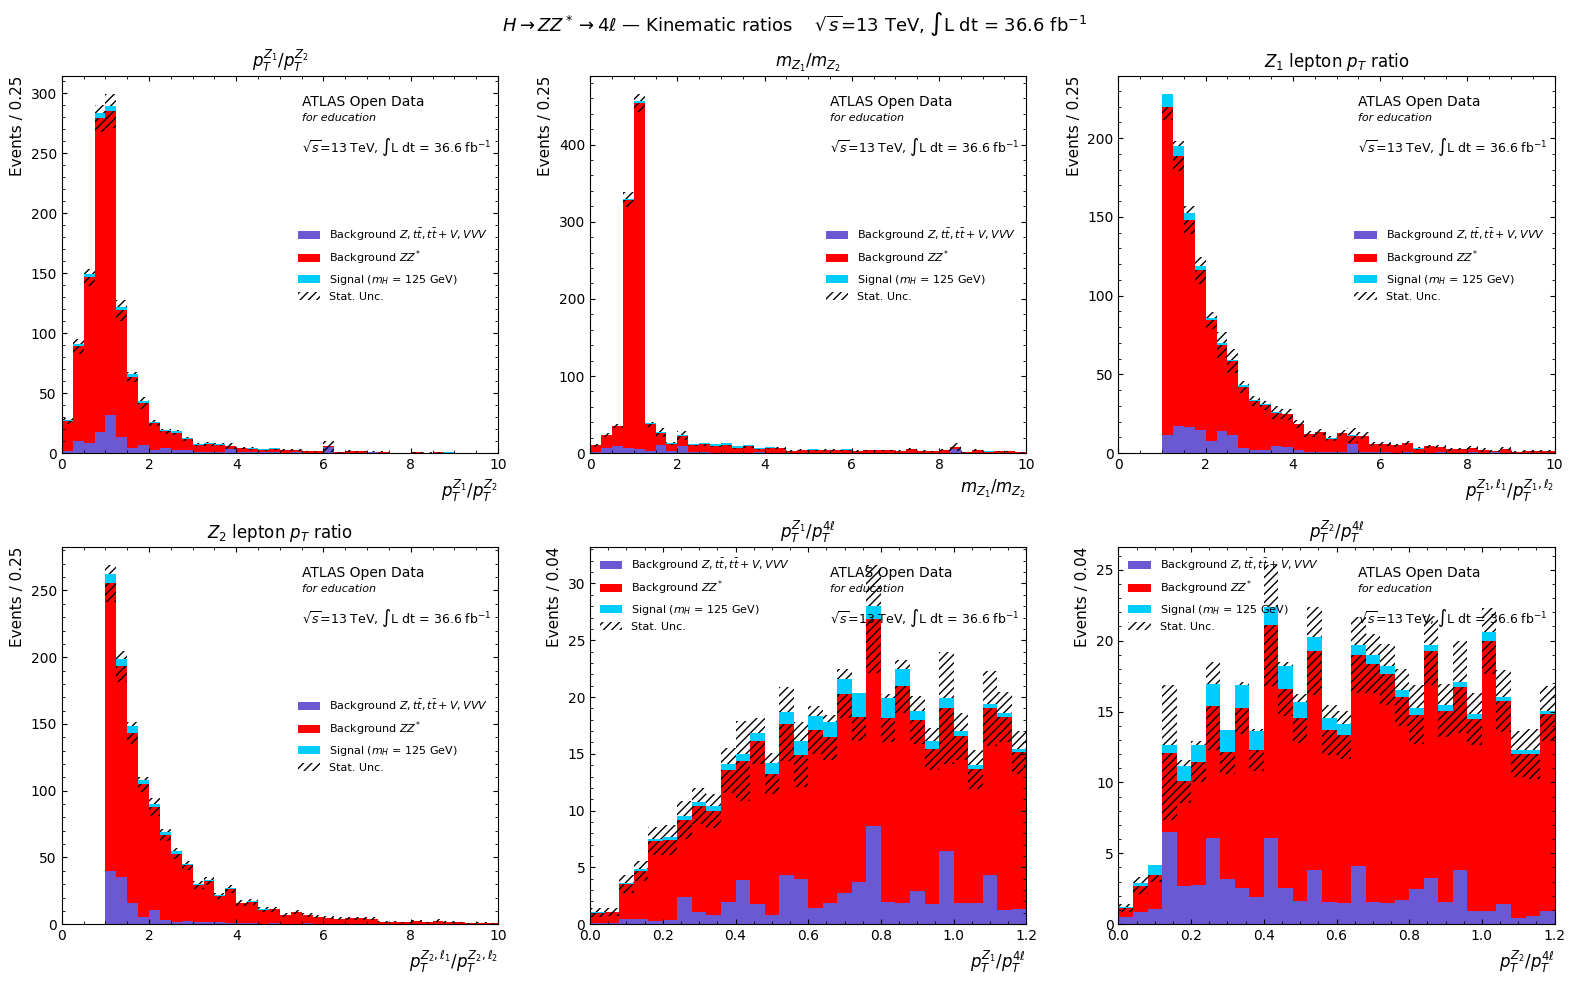
\includegraphics[width=0.28\textwidth]{Figures/download (16).png}\hfill
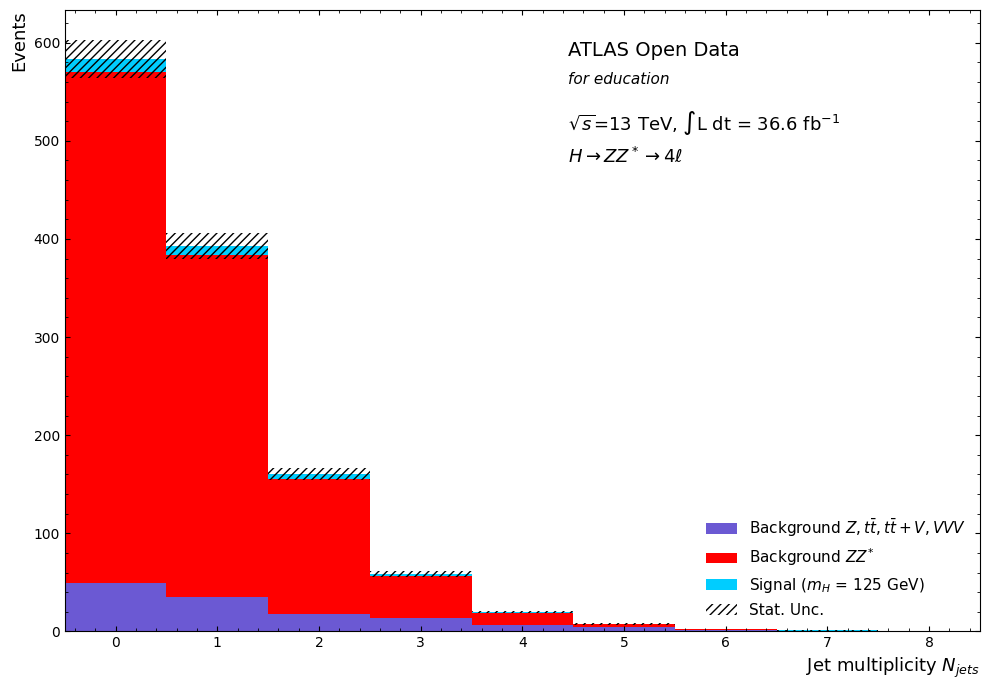
\includegraphics[width=0.28\textwidth]{Figures/download (17).png}\hfill
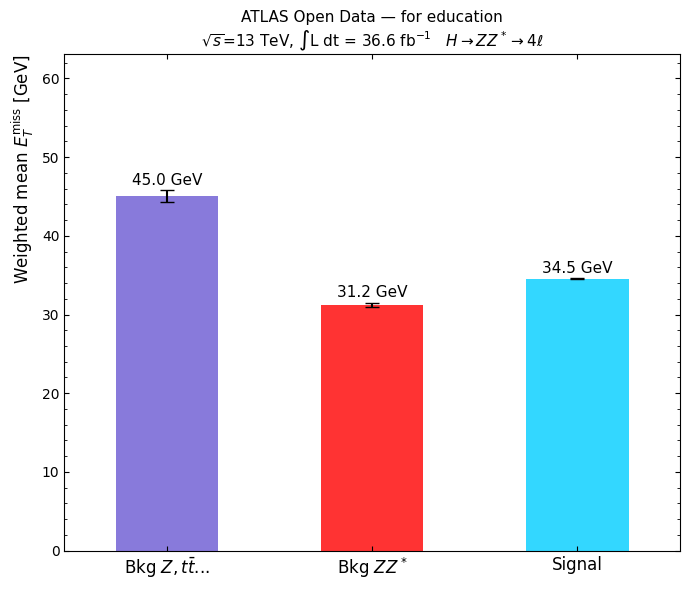
\includegraphics[width=0.28\textwidth]{Figures/download (18).png}

\end{minipage}%
}

\caption{Distribution of the kinematic variables used in the analysis.}
\label{fig:kinematic_variables}

\end{figure*}


\end{document}





















































































































